\section{Experimental sensitivity}
\label{sec:experiment}

Emphasize discovery potential, not just exclusion sensitivity. May be difficult to combine predictions since some collaborations tend to use exclusion-only predictions e.g. SuperCDMS optimal interval. 

\subsection{Prospects for reaching the neutrino fog}
What are the challenges, R\&D needs for mature technologies to reach the neutrino floor?  Are there any new technologies sensitive to this space that can potentially overcome some of these challenges, and might be competitive with the more mature technologies with sufficient investment?
\subsubsection{Currently-funded experiments and R\&D toward next generation}
\label{sec:currentexperiments}

\begin{figure}
    \centering
    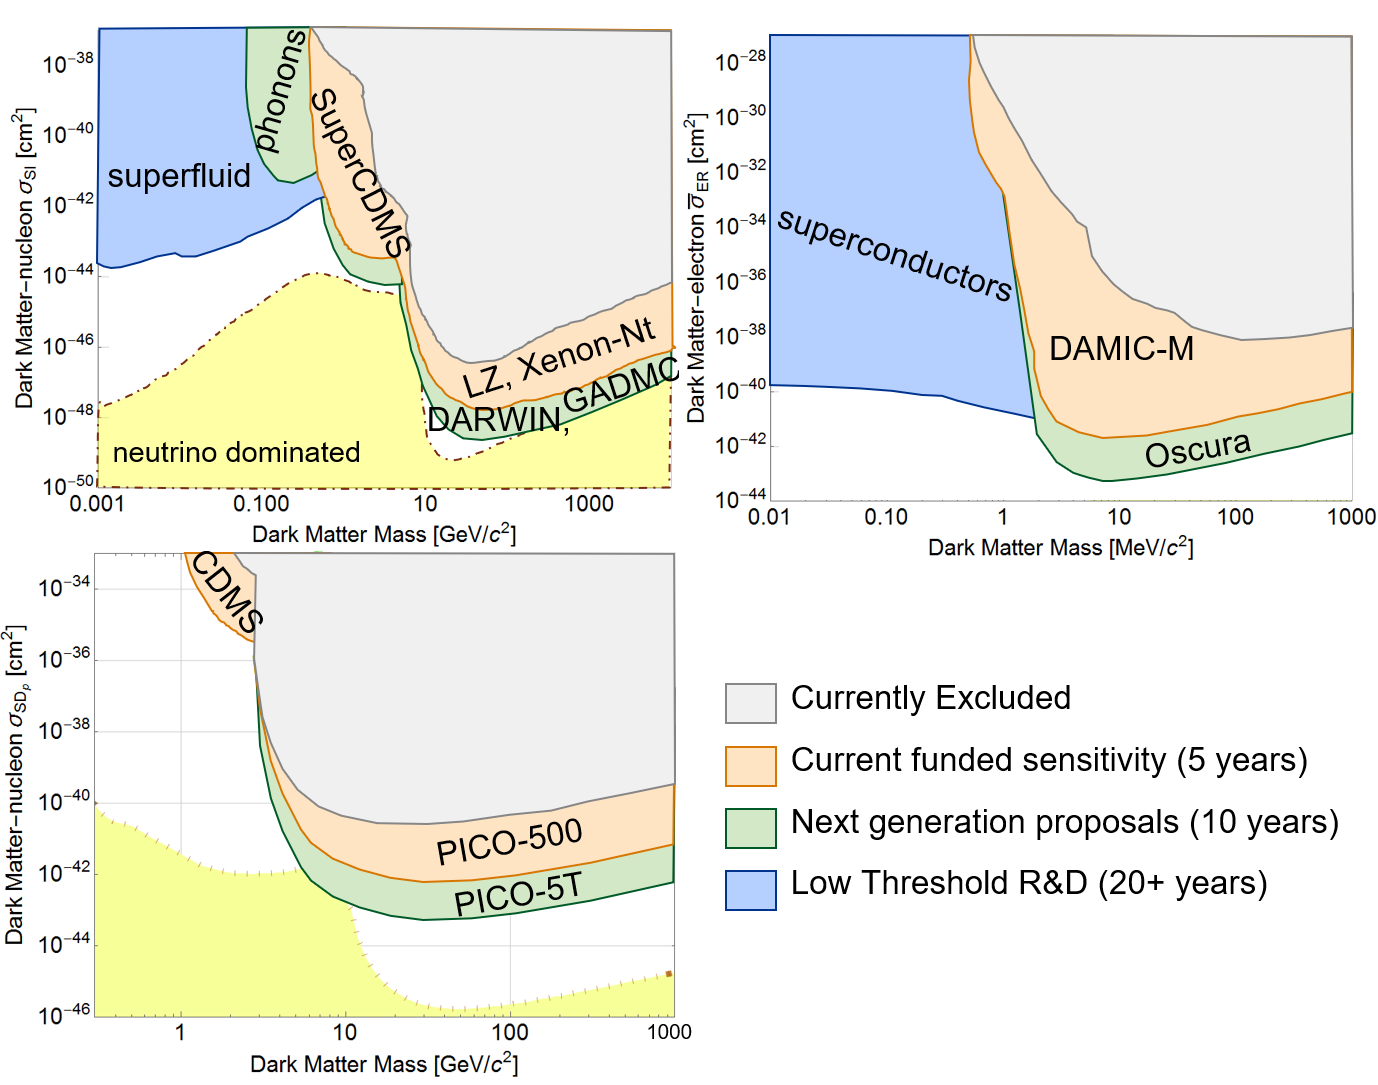
\includegraphics[width=\textwidth]{figures/wimp_sensitivty_cartoon.png}
    \caption{Currently excluded generic spin-independent NR, spin-dependent NR, and ER cross sections. Projected sensitivity of near- amd medium-future experiments. Probably need ER absorption too. Current version is a cartoon and NOT indicative of experiments, labels, timescales, etc.}
    \label{fig:si_sensitivity}
\end{figure}

%Prisca: What would be the umbrella theory here?  Perhaps that belongs in the motivation area of the introduction and we should nest the theory with the type of search (e.g. NR, ER scattering, ER absorption, Dark sector, etc) OR are you imagining that this is basically just a laundry list of what might be searched for?

\paratitle{Liquid Xenon} 
Liquid Xenon (LXe) is an ideal target for rare event detection, and is particularly well suited for WIMP searches. Xenon is an excellent scintillator, highly transparent to its own scintillation light. It is readily available on the market with a typical world production rate of about 65 tonnes/year. Xenon can be effectively purified for particle detector applications in the multi-tonne range. The high density of LXe allows for the construction of compact detectors that feature a low-background inner core due to the large atomic number of xenon and the absence of significant long-lived radioisotopes. The mean free path of high-energy gamma rays from natural radioactivity in detector materials is typically much smaller than the detector size, so that the former interact in the outermost region of the target (self-shielding), enabling for their efficient removal in offline data analysis. When combined with a technology capable of position reconstruction, namely a two-phase Time Projection Chamber (TPC), this allows the definition of a low-background inner fiducial volume that is used for rare event searches.

\begin{figure}[!htbp]
\begin{center}
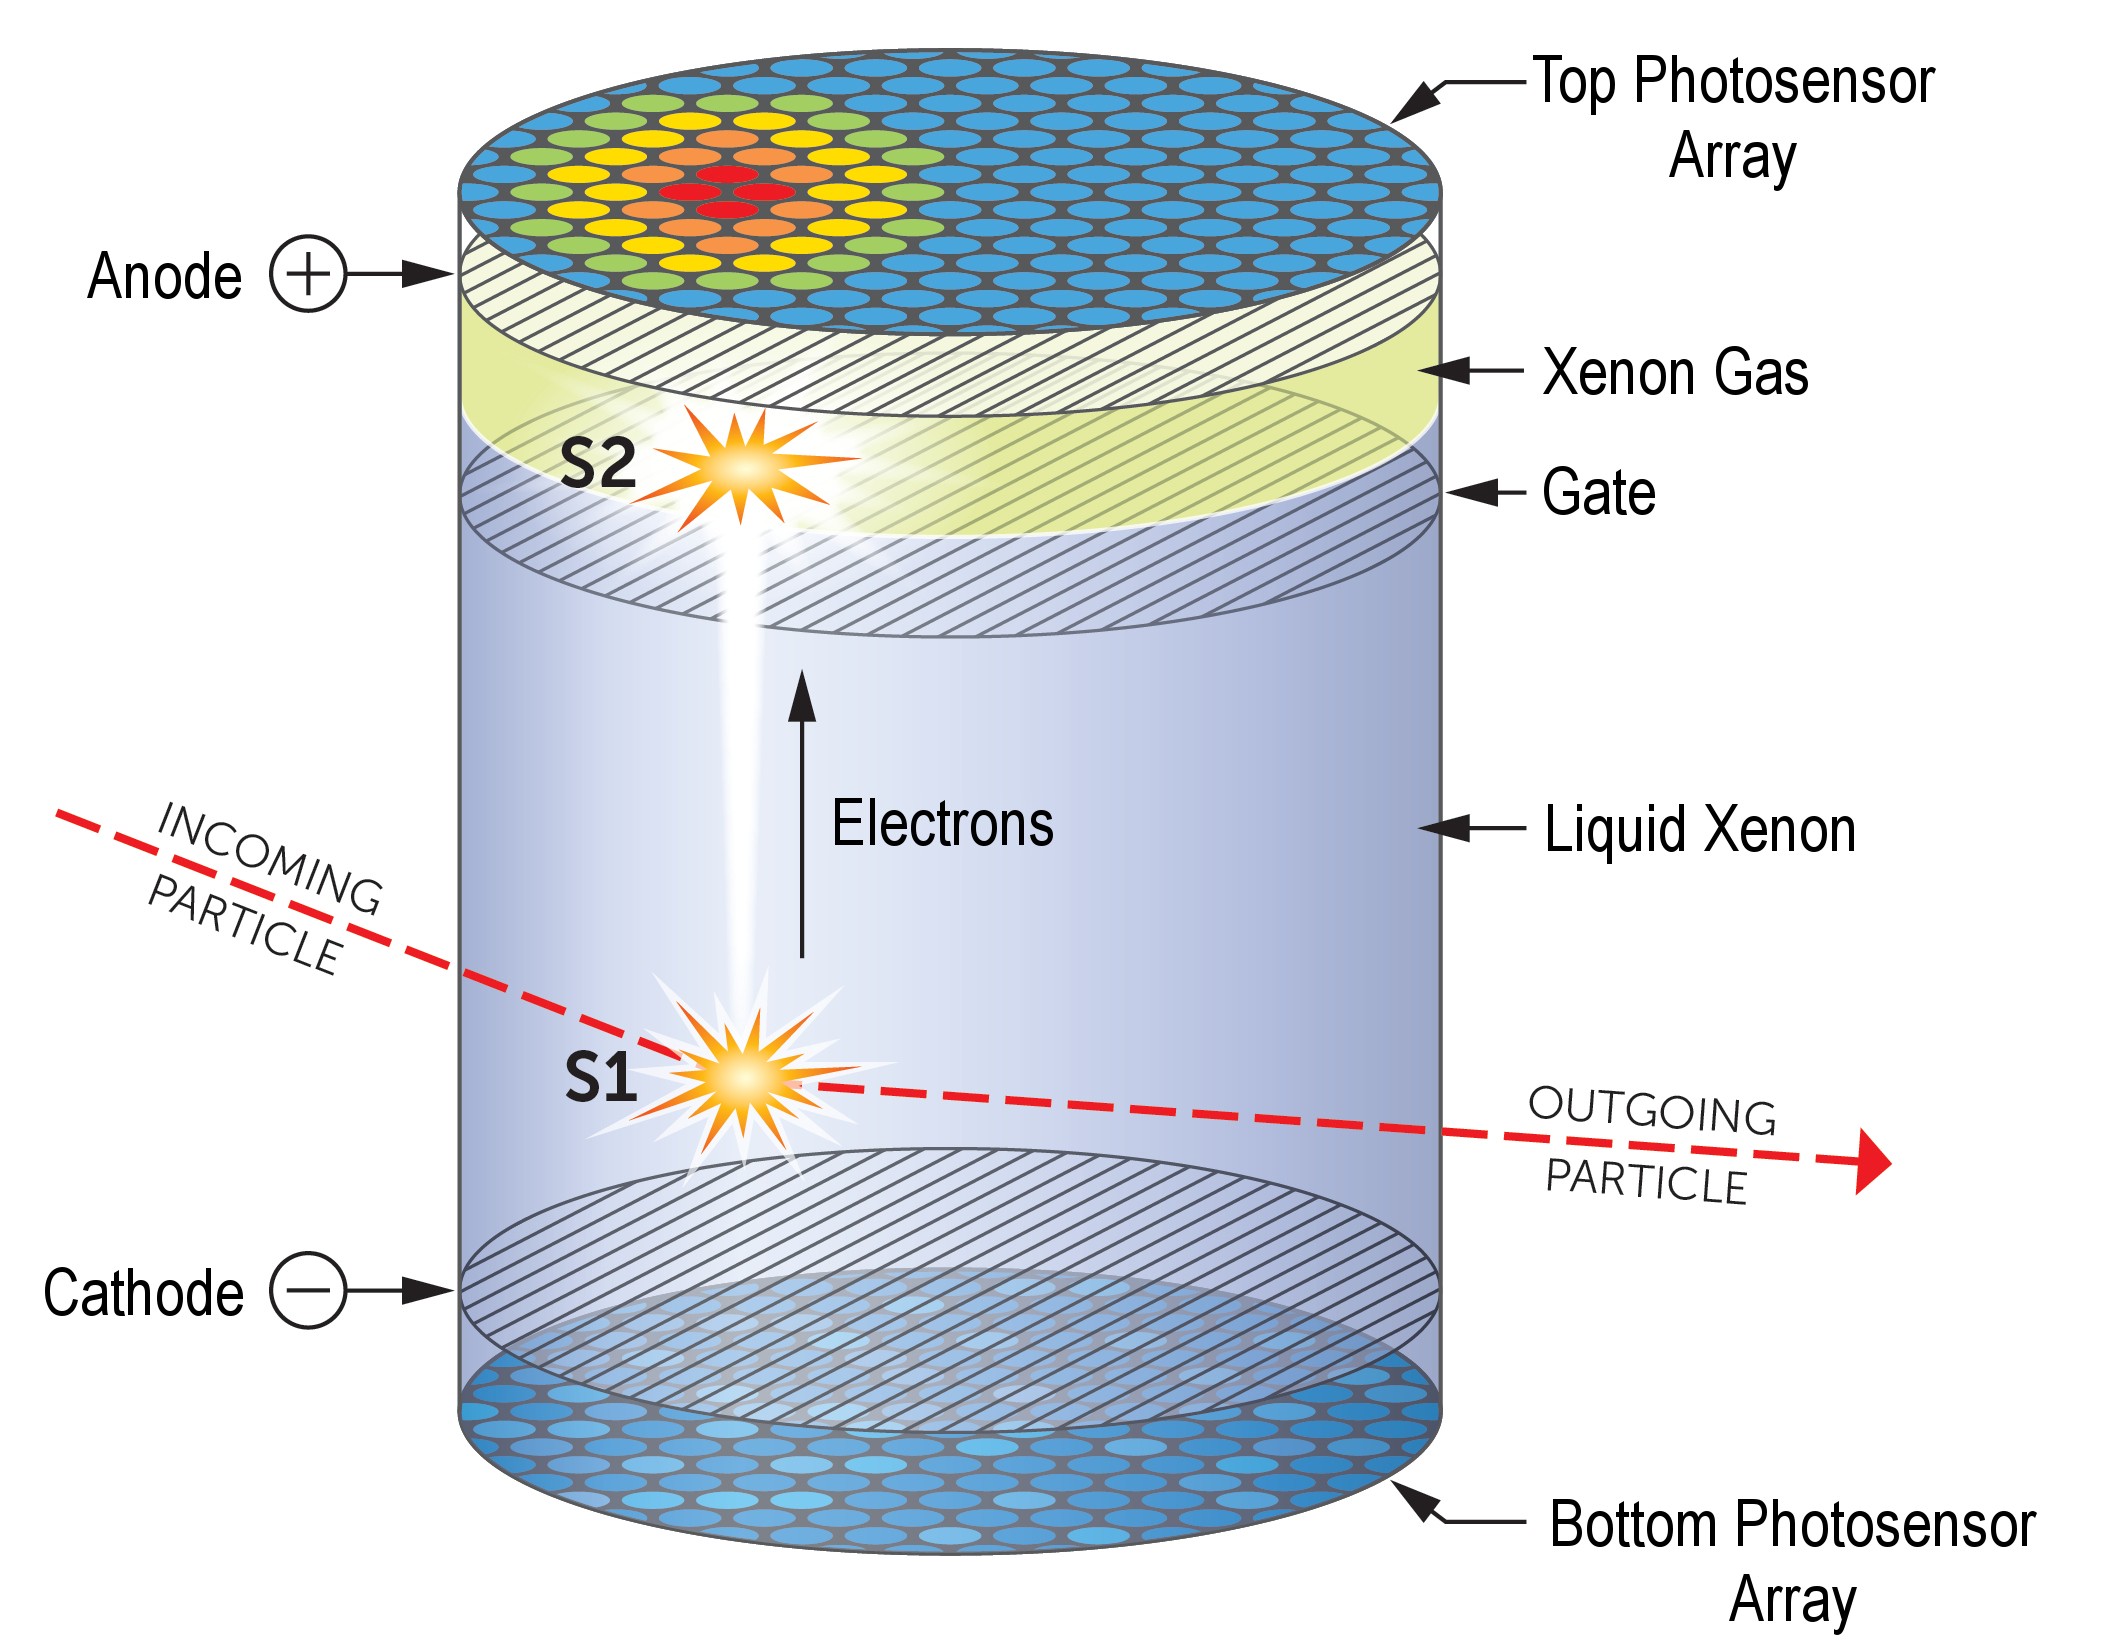
\includegraphics[width=0.99\columnwidth]{figures/xenon_fig_tpc-mo_lifton.jpg}
\caption{Principle of a dual-phase liquid xenon time projection chamber. Energy from a particle interaction within the active liquid xenon volume produces prompt scintillation light (S1) and a delayed  signal (S2) from electroluminescence (proportional scintillation) in the gaseous xenon layer. The localization of the S2 signal and the time difference between S1 and S2 allows for determination of the original vertex location.}\label{fig:tpcsketch}
\end{center}
\end{figure}


The LXe two-phase time projection chamber technology combines the 3D-position reconstruction capabilities of traditional single phase noble liquid TPCs~\cite{Rubbia:1977zz} with low ionization sensitivity, enabled by emission detector designs~\cite{osti_4101722}. The typical layout of a LXe two-phase TPC is sketched in Fig.~\ref{fig:tpcsketch}. The xenon gas contained in a cryostat is kept at its boiling point ($\approx$-100$^\circ$C) to ensure the co-existence of the liquid and gas phases, with a small gas pocket located above the active LXe volume. The target is instrumented with a set of optically transparent electrodes that establish electric fields in the LXe volume (50-600~V/cm) and across the liquid/gas interface (8-10~kV/cm). An interaction in the LXe target excites and ionizes the xenon atoms, giving rise to a prompt VUV scintillation signal (S1), which is read out by two arrays of cryogenic photosensors. In the presence of electric fields, a fraction of the ionization electrons survive recombination and drift towards the gas pocket. The higher electric field at the liquid/gas interface extracts the electrons from the liquid surface and produces electroluminescence light (S2), read out by the same set of photosensors. The simultaneous measurement of S1 and S2 enables precise 3D position reconstruction of individual interactions, allowing definition of the inner fiducial volume, as well as distinguishing single-site from multi-site interactions. The ratio of the S2 and S1 signal amplitude depends on the nature and energy of the primary ionizing particle, further allowing to discriminate between electron recoils and nuclear recoils. Discrimination powers of $>$99.7\% have been demonstrated down to 2\,keV$_R$~\cite{LUX:2020car}. Lower analysis thresholds can be achieved by dropping the requirement of the presence of an S1.

Figure~\ref{fig:xenon_evolution} summarizes the impressive achievements of the LXe-TPC technology, pioneered in early 2000s by ZEPLIN-II~\cite{ALNER2007287}, ZEPLIN-III~\cite{Akimov:2011tj} and XENON-10~\cite{XENON10:2011prx}. Since then a series of LXe-TPCs of increasing target mass and decreasing background has led the direct detection field across more than 3 orders of magnitude, passing through XENON100~\cite{APRILE2012573}, LUX~\cite{AKERIB2013111}, PandaX-I, and PandaX-II~\cite{pandax} with  XENON1T~\cite{xenon1t} and PandaX-4T~\cite{PandaX-4T:2021bab} presently holding the most stringent constraints for WIMP masses above 2\,GeV/c$^2$ (0.1\,GeV/c$^2$ if the Migdal effect is assumed) in a 1\,tonne$\cdot$year and 0.6\,tonne$\cdot$year exposure, respectively~\cite{PhysRevLett.123.251801, PhysRevLett.123.241803,PandaX-4T:2021bab}.

The PandaX-4T experiment, developed by a Chinese-US collaboration, is still operating at China Jinping Underground Laboratory (CJPL)~\cite{Kang:2010zza}. It features a 3.7~tonne active mass (2.6~tonne fiducial) and, after an initial commissioning run, plans to continue operation until 2025, with an expected exposure of no less than 5.6 tonne$\cdot$year and a nuclear recoil energy detection threshold of 3~keV~\cite{PandaX:2018wtu}.

\begin{figure}[!htbp]
\begin{center}
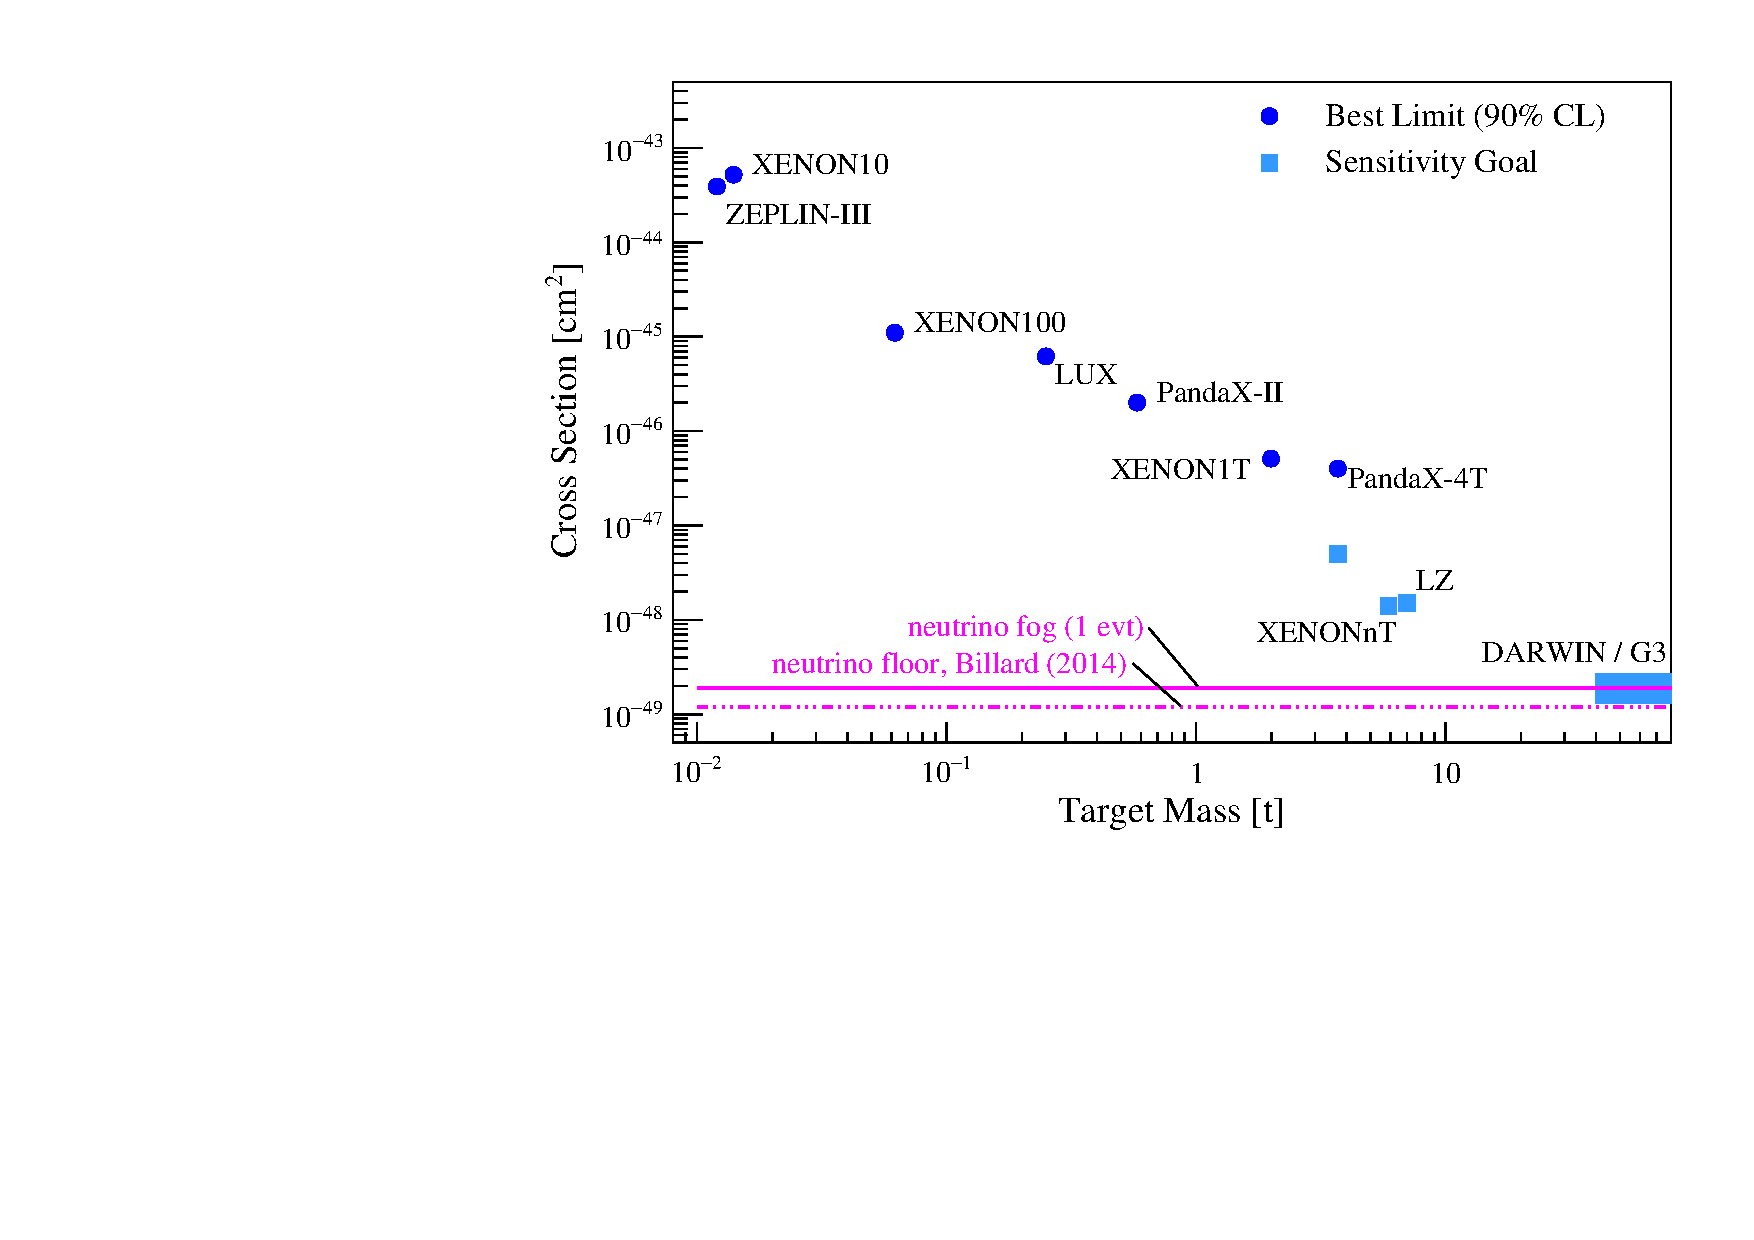
\includegraphics[width=0.48\columnwidth]{figures/xenon_sens_vs_mass.pdf}
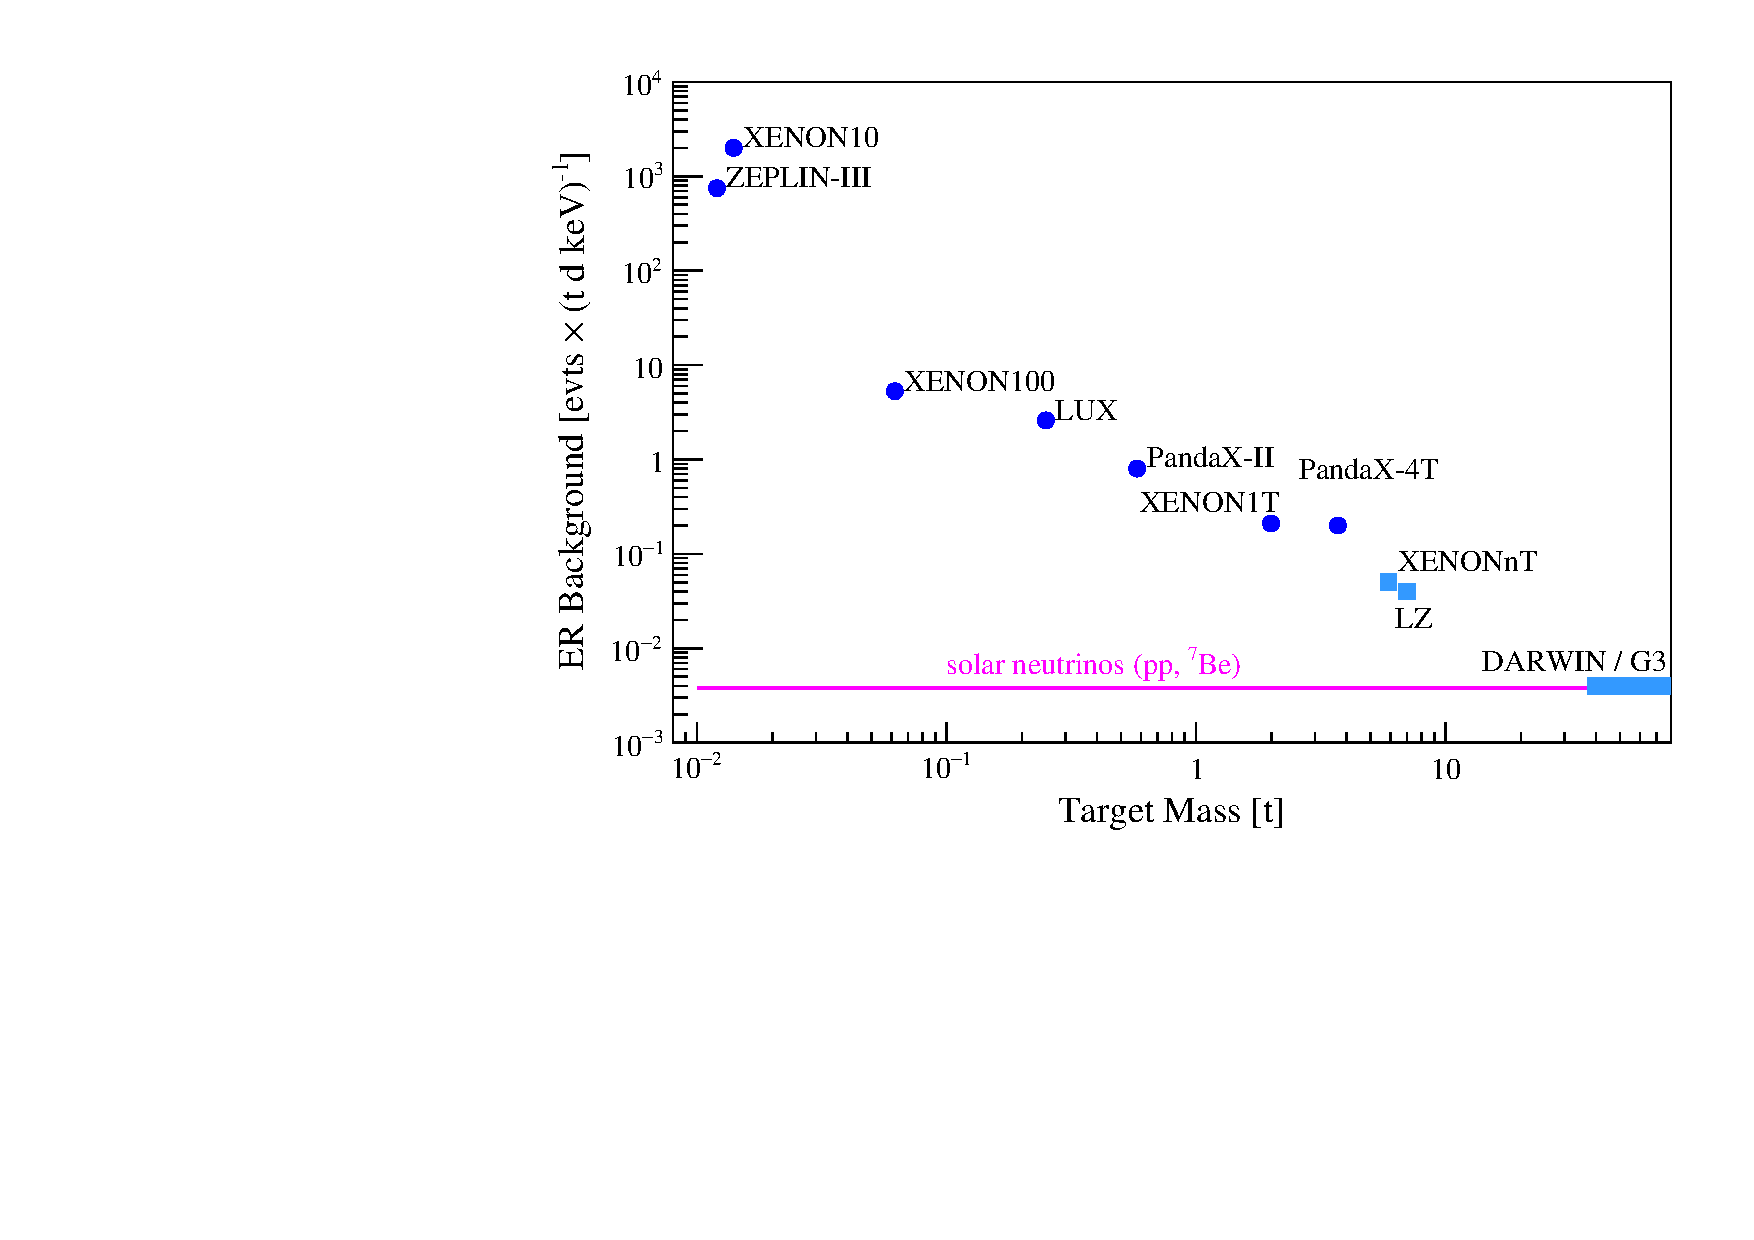
\includegraphics[width=0.48\columnwidth]{figures/xenon_background.pdf}
\caption{Development of the LXe-TPC technology since its inception. The improvement in sensitivity to spin independent WIMP-nucleon coupling achieved by LXe experiments of increasing target masses is shown on the left. The cross section values refers to a WIMP mass of 50~Gev/c$^2$. Sensitivity goals are also reported for experiments that have not yet been completed. The right plot shows, as function of the target mass, the solid progress made in terms of background suppression. The maturity of the technology allowed, at each scale, the identification and characterization of the dominant background sources in the WIMP energy region of interest and the development of techniques capable of efficiently suppressing them for the next phase. Cross section values and background rates are extracted from Ref.~\cite{PhysRevLett.100.021303,PhysRevD.94.122001,AKIMOV201214,PhysRevLett.116.161301,Wang_2020,XENON:2018voc,PandaX:2018wtu,PandaX-4T:2021bab,AKERIB201804,XENON:2020kmp}.
}
\label{fig:xenon_evolution}
\end{center}
\end{figure}

\begin{figure}[!htbp]
\begin{center}
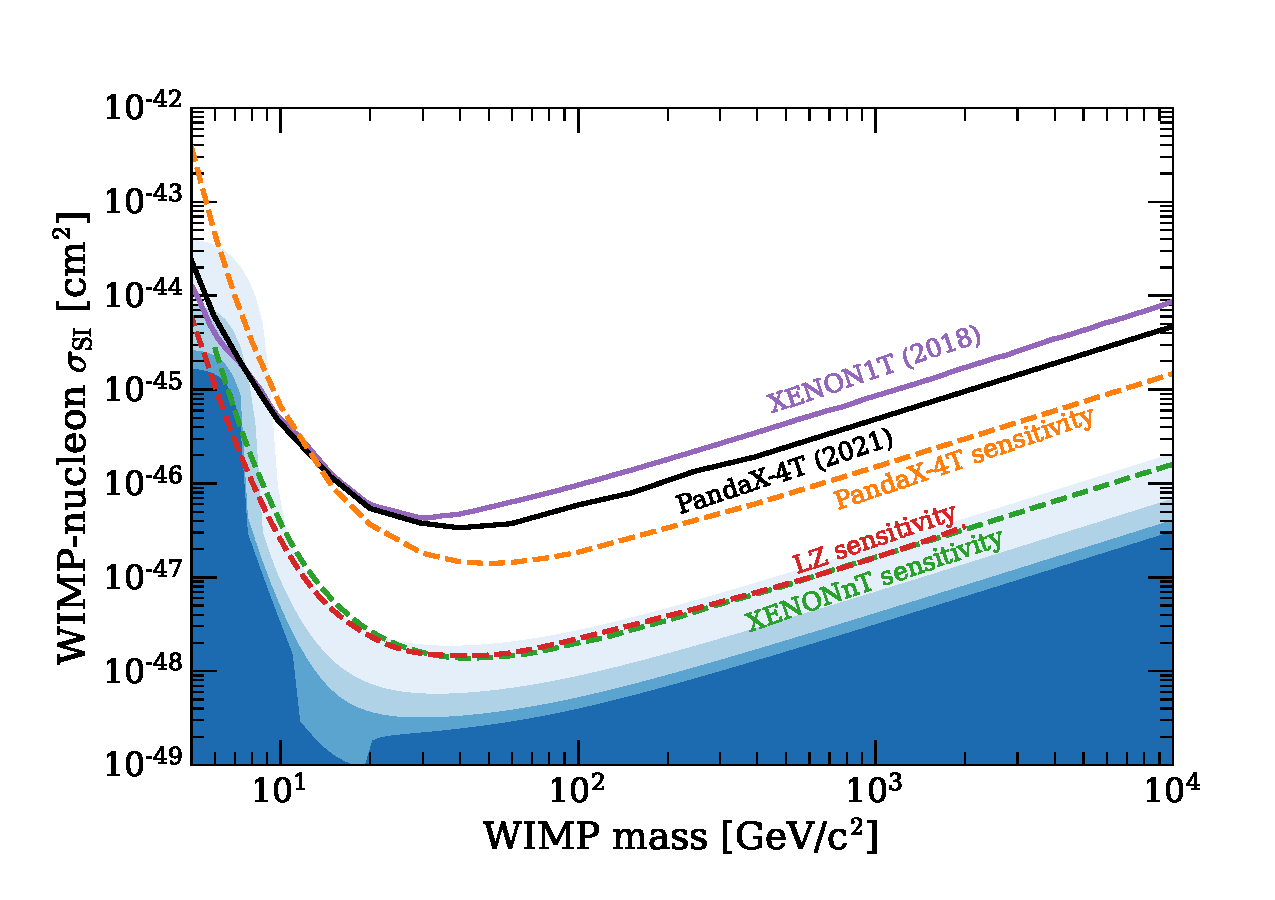
\includegraphics[width=0.99\columnwidth]{figures/xenon_CF1WP1_G2sens_v3.pdf}
\caption{{\color{red}Figure still in progress.} PandaX-4T~\cite{PandaX:2018wtu}, LZ~\cite{AKERIB201804} and XENONnT~\cite{XENON:2020kmp} projected sensitivity to spin-independent WIMP coupling with nucleon compared to XENON1T and PandaX-4T results~\cite{XENON:2018voc,PandaX-4T:2021bab}. The LZ curve is calculated for a 15\,tonne$\cdot$year and with a one-sided upper limit construction. The XENONnT curve is calculated for a 20\,tonne$\cdot$year exposure and with a two-sided interval construction, which is intrinsically less sensitive than the one-sided construction (A 2021 paper authored by members of several dark matter collaborations provided recommendations to ensure that future results are calculated on the same statistical basis~\cite{recommendation_dark_matter}). The PandaX-4T sensitivity is estimated for a 5.6 tonne*year exposure, the PandaX-II detection efficiency, and a cut-and-count signal treatment with 40\% nuclear recoil acceptance~\cite{PandaX:2018wtu}. The blue region represents the neutrino fog, where sensitivity becomes systematics-limited. {\color{red}Refine neutrino fog text after Sec.~2 of this whitepaper has been written.}}
\label{fig:xenon_sensi}
\end{center}
\end{figure}

Two new multi-tonne LXe-TPCs, LZ and XENONnT, are operative since 2021 with a target sensitivity of about 1-2$\times$10$^{-48}$ cm$^2$ (see Fig.~\ref{fig:xenon_sensi}).
The US-European-Japanese collaboration XENON is running the XENONnT experiment at the Laboratori Nazionali del Gran Sasso (Italy). The detector features a 5.9\,tonne LXe target (4.0\,tonne expected fiducial) surrounded by a Gd-doped water Cherenkov active veto to suppress and tag neutron-induced background.

The XENONnT collaboration plans to accumulate a 20\,tonne$\cdot$year exposure. The projected neutrino-induced background rate in the WIMP ROI is of 0.27 events/tonne$\cdot$year and 0.08 events/tonne$\cdot$year for solar and atmospheric neutrino respectively, with the former not affecting WIMP searches for masses larger than 10\,GeV/c$^2$. While the number of events in the WIMP region might be indicative of the background, it does not fully capture the reach of xenon-based detectors where, thanks to the maturity of the technology, the backgrounds are extremely well characterized and modeled in multiple parameter spaces, allowing for a powerful statistical inference process~\cite{XENON:2020kmp}. 
The US-European LUX-ZEPLIN (LZ) experiment is presently operating at Sanford Underground Research Facility (USA) and aims to accumulate a 15\,tonne$\cdot$year exposure~\cite{AKERIB201804}.

The detector features a 7\,tonne target (5.6\,tonne expected fiducial), surrounded by an instrumented LXe skin layer and a Gd-loaded liquid scintillator which together form an efficient anti-coincidence veto and in~situ background monitor. The expected neutrino-induced background rate in the WIMP signal region is 2.35\,events/tonne$\cdot$yr (solar) and 0.02\,events/tonne$\cdot$yr (atmospheric).

About a decade and half of intensive development and deployment has made the LXe-TPC an extremely mature technology capable of being extended to a larger scale with reliable sensitivity projections and consistently solid progress (see Fig.~\ref{fig:xenon_evolution}). Extension of this technology to an even larger scale, enabling systematics-limited exposures, is within reach. A definitive next-generation experiment targeting exposures on the order of 1\,ktonne$\cdot$year would fully explore the accessible WIMP parameter space. The strategy towards such an experiment will be informed by outcomes from the current projects, complemented by a limited and well-defined set of R\&D activities that should take place concurrently. The needed technological improvements appear modest given the limited scale-up that is required with respect to current experiments, less than a factor of two in linear dimensions. 

In China, PandaX-4T is expected to be gradually upgraded into a multi-ten-ton experiment with a nominal fiducial target of 30~ton, to push the sensitivity to dark matter-nucleus coherent scattering to the “neutrino fog” for dark matter masses above 10~GeV/$c^2$. The PandaX collaboration is actively pursuing R\&D for the next generation experiment in parallel with the operation of PandaX-4T until 2025, after which the upgrade is expected to start.

The DARWIN collaboration~\cite{DARWIN:2016hyl}, a successor to XENON, has already started in Europe an intense R\&D program. Given their current leadership roles and expertise, the US teams in both XENONnT and LZ (about 50\% of the community) are well-positioned to contribute significantly to this next-generation effort; in fact, there would be substantial opportunity cost in delaying the US engagement. In 2021, scientists in the LZ and XENON/DARWIN collaborations formally expressed their intent to join forces towards towards this next-generation xenon-based experiment, pursued by a single, joint scientific collaboration~\cite{mou}. While development of a detailed strategy is underway, one potential path forward would foresee a staged project minimizing technological risk at reduced cost, while increasing scientific productivity with an accelerated timeline. A detector design that can be extended along the drift direction would bring substantial benefit:
\begin{itemize}
    \item Minimized technological risk: It would allow in the early phase the operation of a detector that, although compact in its drift direction, would feature full-size electrodes and photo-detector arrays, enabling their characterization directly at the final scale and condition.
    \item Accelerated time to scientific return: It would allow operation of the compact version of the detector, while the full xenon inventory is being procured. 
    \item Reduced cost: A less aggressive timeline for the xenon procurement would enable a meaningful reduction of the project costs, by minimizing impact on the market price of xenon.
    \item Broad user base: It would allow early characterization of the various sources of background in a low background environment, as well as an early science program, to fully engage the next generation of scientists. 
\end{itemize}

The support for a next generation xenon-based experiment extends beyond the new DARWIN/XENON/LZ and PandaX collaborations, as witnessed by the long list of approximately 600 authors signing a recent community white paper outlining the physics reach of such an experiment~\cite{whitepaper_on_the_arxiv_still_in_february}. The large detector scale and low background, combined with many advantageous properties of xenon properties as target, enable a rich science portfolio that extends well beyond WIMPs, transforming such a detector into a cost-effective, broad, low-background astroparticle physics observatory. 

\paratitle{Liquid Argon} 
DEAP Lead:


%DarkSide lead: Graham Giovanetti


The successful campaign of the DEAP-3600 experiment demonstrates the feasibility of multi-tonne-scale LAr detectors, including the development and use of ultra-high purity acrylic~\cite{amaudruzDesignConstructionDEAP36002019a} and novel techniques for achieving heavily suppressed Rn contamination. Thanks to its large size, DEAP-3600 also demonstrated the promise of large-scale LAr detector for searching for dark matter at the highest masses, up to the Planck scale~\cite{deapcollaborationFirstDirectDetection2022}.  DarkSide-50 demonstrated the sensitivity of a LAr TPC using Underground Argon (UAr), heavily depleted in $^{39}$Ar, to light dark matter with nuclear~\cite{darksidecollaborationLowMassDarkMatter2018} and electronic~\cite{thedarksidecollaborationConstraintsSubGeVDarkMatter2018} couplings. This is due in part to the relatively light argon nucleus and to the high degree of chemical purity achievable in LAr due to its cold temperature.  The DarkSide-LowMass experiment is now being planned to leverage these advantages to search for dark matter with cross sections down to the solar neutrino fog with an estimated tonne-year exposure of further-depleted UAr.

The DarkSide-20k (DS-20k) experiment of the multinational Global Argon Dark Matter Collaboration (GADMC) will search for dark matter using an UAr target instrumented as a dual-phase time projection chamber (TPC)~\cite{Aalseth:2018gq}.  The GADMC includes more than 400 scientists from over 60 institutions, mostly coming from the ArDM, DarkSide-50, DEAP-3600, MiniCLEAN, and XENON collaborations, and DS-20k will inherit successful elements from these experiments. These include the use of UAr, which DarkSide-50 demonstrated to have an $^{39}$Ar concentration at least 1400 times smaller than atmospheric argon~\cite{Agnes:2015gu,Agnes:2016fz,Agnes:2018ep}, and a radiopure acrylic structure, a technology pioneered by the DEAP-3600 experiment~\cite{Nantais:2013jp,Amaudruz:2018gr}.  The TPC is designed to take advantage of the favorable properties of liquid argon, including demonstrated electron recoil background discrimination power better than $10^8$~\cite{Adhikari:2021} and excellent chemical purity~\cite{Ajaj:2019jx,Ajaj:2019jk}, and operate with $<0.1$ background events within the 20.2~t fiducial volume over a ten year run, other than an expected ($3.2 \pm 0.6$) events from coherent neutrino scattering.  The DS-20k experimental apparatus consists of three nested detectors installed within a membrane cryostat nearly identical to the two existing ProtoDUNE cryostats~\cite{Abi:2020gv,Abi:2020hj,Abi:2020je}: the inner two-phase argon TPC, a neutron veto, and an outer muon veto. The apparatus will be located in Hall C of the Gran Sasso National Laboratory (LNGS). The DS-20k UAr target will be extracted by Urania~\cite{Aalseth:2018gq}, an argon extraction plant capable of extracting 330~kg/d of UAr, and purified with the Aria plant~\cite{Agnes:2021us}, a 350~m cryogenic distillation column designed to separate argon and other rare stable isotopes.  As illustrated in Fig.~\ref{fig:limitplot_SI}, DarkSide-20k experiment extends the cross section vs. mass range sensitivity in the search for dark matter to  $4.6\times 10^{-48}$\,cm$^2$ for a 90\% C.L. exclusion (and $1.5\times 10^{-47}$\,cm$^2$ at a $5\sigma$ discovery significance) for a 1\,TeV/$c^2$ WIMP, well beyond any current or presently funded experiment.  This will lead to either discovery, confirmation, or exclusion of the WIMP dark matter hypothesis down to the level where coherent scatters from atmospheric neutrinos become an irreducible background.  DarkSide-20k will also be sensitive to a galactic supernova neutrino burst originating anywhere in the Milky Way Galaxy~\cite{Agnes:2021ke}.

The ultimate objective of the GADMC is the construction of the Argo detector, which will have a 300~t fiducial mass and will push experimental sensitivity into the atmospheric neutrino fog.  The excellent electron recoil (ER) rejection possible in argon will eliminate backgrounds from solar neutrinos, which will extend the sensitivity of Argo beyond that of technologies with more limited ER discrimination.  Such a large detector would also have excellent sensitivity to a neutrino burst associated with a galactic supernova~\cite{Agnes:2021ke}.  If located at SNOLAB or at similar depth, Argo will also have the potential to observe CNO neutrinos for the first time and solve the Solar Metallicity Problem~\cite{Agnes:2020wd,Franco:2016ex}.  The further expansion of several technologies are critical for the success of Argo. The continued development and operation of Urania~\cite{Aalseth:2018gq} and Aria~\cite{Agnes:2021us} would enable 400~t of UAr to be extracted and purified over a period of about five years. Facilities for the long-term underground storage and assay of this argon are also needed. The Argo detector will be instrumented with more than 100~m$^2$ of photodetectors. This would be greatly simplified by the continued evolution of the large-area SiPM-based photosensors developed for DS-20k~\cite{DIncecco:2018hy,DIncecco:2018fx} into digital SiPMs, which would reduce the quantity of cables, significantly reduce noise, and decrease the background rate in the detector. Finally, all future detectors entering into the neutrino fog would benefit from improved atmospheric neutrino background modeling, which currently dominates the uncertainty on the experimental sensitivity.

\paratitle{Solid State} 
The Super Cryogenic Dark Matter Search (SuperCDMS) SNOLAB experiment is a 2$^{nd}$ generation dark matter experiment, which will commission its solid-state detectors 2 km underground at the SNOLAB facility in Sudbury, Canada.  The solid-state detectors are germanium or silicon crystals patterned with both Quasiparticle-assisted Electrothermal-feedback Transition edge sensors (QETs) as phonon sensors and electrodes used for charge readout and/or biasing the crystal.  The patterned QETs and electrodes are optimized to operate as either High Voltage (HV) or interleaved Z-dependent Ionization and Phonon (iZIP) detector.

In an HV detector, the electrodes are used to apply a relatively large bias voltage across the crystal.  The applied voltage gives rise to an \textbf{E}-field that causes electrons and holes to drift to opposing faces of the detector. As they move through the crystal, the charges scatter off the lattice, generating additional phonons via the Neganov-Trofimov-Luke (NTL) effect ~\cite{Neganov1985, Luke1988}.  The resulting total energy observed by the QETs on the detector faces is $E_{tot} = E_r + N_{eh}eV_{b}$, Where E$_r$ is the initial recoil energy, and N$_{eh}$ is the number of electron-hole pairs initially created. These devices have an improved ultra-high resolution and reach lower thresholds allowing them to probe lower DM masses.  The HV detectors are expected to explore WIMP DM masses down to ~0.3 GeV. 

In an iZIP detector, a low voltage bias is applied in order to minimize the NTL effect. The electrodes are also used as charge collectors.   iZIP detectors therefore measure both prompt phonons and ionization charge signals, which can be used to perform ER/NR discrimination based on the difference in ionization yield. Furthermore, optimization of the electrode layout allows identification of surface events via a charge signal collection asymmetry: bulk (nominally symmetric signals) and surface (highly asymmetric signals) events.  This allows rejection of beta particles and further reduces the background in the operation of these devices. The advanced rejection capabilities of these devices project sensitivities in a ``background-free'' mode to WIMPs with masses $>$5 GeV and in a “limited-discrimination” mode to WIMPS $>$1 GeV~\cite{SCDMS2017}.

The SuperCDMS SNOLAB experiment anticipates observing approximately 50 events associated with neutrino interactions, but will not reach the neutrino fog.  The background and detector improvements needed to reach the fog have been identified as part of a near-term SuperCDMS upgrade plan.  Backgrounds improvements include sourcing new material, replacing components with lower background alternatives, and improving detector fabrication/tower assembly to reduce the $^{210}$Pb plated onto the surface from radon, all within a reasonable cost for implementation.  Proposed detector upgrades common to both HV and iZIP style detectors include: 1) smaller detector sizes; 2) lowering the TES critical temperature (T$_C$); and 3) improving phonon transmission across interfaces.  Scaling to smaller detectors will improve the phonon/ionization resolution of the SuperCDMS detectors, which in turn will improve rejection of bulk ER backgrounds. This development is reasonably mature with prototype Si HVeV detectors (an HV style device) already deployed at test facilities ~\cite{SCDMS2019,SCDMS2020}.  R\&D efforts are set to shift toward the development of a Ge HVeV detector and optimization of these devices.  Lowering of the TES T$_C$ is less mature, but a viable path forward is known. The thin tungsten film that is at the heart of the QET can grow in two different phases, $\alpha$-W with a T$_C$ of 15 mK or $\beta$-W with a T$_C$ over 2 K, during deposition. By mixing these two phases in different ratios the T$_C$ can be tuned between the two extremes.  The challenge is in identifying the proper deposition parameters under which the W film will grow at the proper ratio in a reproducible and controllable manner.  Improvements in phonon transmission from the crystal all the way to the W TES is the least mature advancement being considered, with no immediate avenues forward identified.
CCDs Lead:



\paratitle{Freon Bubble Chambers} 
PICO Lead: Alan Robinson

The PICO Collaboration uses freon-filled bubble chambers for nuclear recoil detection in targets with high spin-dependent and low spin-independent cross-sections, allowing the exploration of orders-of-magnitude more dark matter parameter space before reaching the neutrino fog than can be achieved in Si, Ge, and noble-liquid targets.  There is strong physics motivation for freon bubble chambers out to kiloton-year exposures and beyond, exposures that are plausible with this technique thanks to its field-leading electron recoil rejection ($O$(1) in $10^{10}$ ER events misidentified as dark matter~\cite{PICO:2019rsv}) and monolithic liquid target.  Past PICO experiments at SNOLAB have reached exposures of $\sim$3~ton-days~\cite{PICO:2019vsc}, including a zero-background (observed) ton-day exposure at 3.3-keV threshold~\cite{PICO:2017tgi}.  The PICO-500 experiment, funded by the Canada Foundation for Innovation, will reach an exposure of XXX ton-years on a C$_3$F$_8$ target by 20YY, including XXX ton-years at ZZ-keV threshold, giving NN expected solar neutrino CE$\nu$NS events, followed by XXX ton-years above the $^8$B CE$\nu$NS endpoint.  This results in a spin-dependent WIMP-proton sensitivity commensurate with the spin-dependent WIMP-neutron sensitivity expected from Generation-2 LXe-TPCs.  Unlike the Generation-2 LXe-TPCs, however, PICO-500's projection is still four-orders-of-magnitude \emph{above} the C$_3$F$_8$ neutrino fog.

1-2 paragraphs (plus cross-reference to IF-08) discussion of instrumentation R\&D enabling the larger bubble chambers needed to explore this parameter space after PICO-500.



\paratitle{Liquid-Noble Bubble Chambers} 
% SBC Lead: Eric Dahl

The Scintillating Bubble Chamber (SBC) Collaboration uses liquid-noble bubble chambers to extend the nuclear/electron recoil discrimination capability of freon-filled chambers to the sub-keV thresholds needed to reach the neutrino fog at 1~GeV.  Liquid-noble bubble chambers differ from their freon-filled cousins in two (related) ways. First, the scintillation coincident with bubble nucleation in the target allows event-by-event energy reconstruction~\cite{Baxter:2017ozv}, which can be used to reject of backgrounds above the few-keV scintillation detection threshold.  Second, noble liquids can be superheated to a far greater degree than molecular fluids, showing sensitivity to sub-keV nuclear recoils while remaining completely insensitive to electron-recoil backgrounds~\cite{Durnford:2021cvb}.  The combination of scalability, low threshold, and background discrimination \emph{at low threshold} gives the noble-liquid bubble chamber unique capability to explore the neutrino fog in the 1--10~GeV WIMP mass range.

The ultimate threshold reach of the liquid-noble bubble chamber is not yet known.  A 10-kg LAr bubble chamber (also capable of operation with LXe) has been built at Fermilab to resolve this question, designed to probe thermodynamic thresholds as low as 40~eV and accomplish nuclear recoil sensitivity calibrations with $O$(10)-eV resolution.  This device is now being commissioned, and low-threshold calibrations will begin in 2023.  Meanwhile, the Canada Foundation for Innovation has funded the construction of a twin 10-kg device for SBC's first dark matter search \cite{Giampa:2021wte}, which has received GW1 approval at SNOLAB.  At a 100-eV nuclear recoil detection threshold (SBC's benchmark until the calibration campaign is complete), this 10-kg LAr chamber will observe 2.5 solar neutrino CE$\nu$NS events per live year.  A follow-up 100-eV threshold LAr experiment at the scale of PICO-500 (1-ton-year exposure) will be sufficient to explore the neutrino fog to $n=2$ at 1-GeV WIMP mass. 


\subsubsection{New technologies}
\paratitle{Super-cooled detectors} 
The snowball chamber is a nascent technology which is analogous in operational principles to superheating in bubble chambers and supersaturation in cloud chambers, except that it relies on supercooling~\cite{szydagis2021}.  The first prototype was constructed by Profs. Levy and Szydagis with students at UAlbany SUNY and shown to likely be sensitive to nuclear recoils from neutrons as the radioactive calibration source, with low sensitivity to electron recoils, as in dark matter bubble chambers~\cite{PICO:2019vsc}. The detector relies on lowering the temperature of liquid water below its freezing point in a sufficiently clean and smooth container so that it becomes metastable instead of immediately solidifying.  An incoming particle such as a dark matter WIMP should be able to trigger the phase transition, and potentially encode directionality as well via the intense hydrogen bonding of water.  Advantages of this technique would be the potential for sub-keV energy threshold and the use of water (for scalability, ease of purification, background neutron moderation, and excellent spin-dependent-proton sensitivity).  If the threshold is indeed as low as claimed for decades for supercooled water in atmospheric sciences, then even only a few kg deployed underground for only a few years could lead to world-leading sub-GeV limits for both the standard SI and SD-proton operators.

In order for this detector technology to become viable, numerous challenges will need to be overcome.  The water volume will need to be sufficiently purified in order to achieve a low energy threshold by lowering the temperature sufficiently without nucleation sites present; reduction in background nucleation through these mitigations, combined with faster reheating methods post-event, should lead to the required livetime of $>$50\%; calibrations of backgrounds from all sources will need to be performed, using betas and gamma-rays to fully characterize the electronic recoil discrimination power, as well as alphas to determine how much Radon contamination would be an issue, and these calibrations would need to be performed as a function of temperature (and pressure) with the goal of finding a “sweet spot” temperature.

With most of the materials, equipment, and supplies exist already through earlier seed-funding initiatives, even for building a larger-scale (only grams tested thus far) viable dark matter experiment that is ready for underground deployment, the required resources for construction would be limited, and the funding agencies will need to take a risk on a new idea that is not only an extrapolation from existing concepts: the cost is low so the risk is low, but the return high, based on the advantages discussed earlier.
\paratitle{Low Background DUNE module} 
Work is underway to explore the feasibility of a low background kTon-scale liquid argon time projection chamber in the context of the Deep Underground Neutrino Experiment (DUNE).  The DUNE program consists of modules, and though the designs for the first two modules have been selected, the third and fourth (the `modules of opportunity’) remain to be determined.  A recent community effort~\cite{SnowmassLowBgDUNElikeWP} explored the option of making one of these a dedicated low background module, with possible sensitivity to high mass WIMPs~\cite{Church_2020}.  This detector could also confirm a galactic WIMP signal discovered in the generation two detectors using an annual modulation.  

This DUNE-like detector would adapt the standard vertical drift design, with the addition of an optically isolated inner volume where increased light detection allows improved energy resolution at low energies and pulse shape discrimination for background reduction.  The detector would take advantage of the significant self-shielding of the liquid argon to reduce the backgrounds in a 3 kton fiducial volume (compared to 10 ktons in the full module).  Use of low radioactivity underground argon reduces the argon-39 and argon-42 internal backgrounds.

The primary research and development challenges for this detector design are associated with the large scale; in general, the radioactive background requirements are less strict than dedicated dark matter experiments.  Quality control of an assay program will need to be strict to ensure the large amount of material meets requirements.  Radon purification and emanation control in large amounts of liquid argon will need to be demonstrated.  Cleanliness controls for a large detector assembled underground will need to be developed and demonstrated.  Current known underground argon sources are not large enough to supply a detector of this size, and the collaboration is in discussion with commercial gas producers to determine whether a cost-effective supply can be achieved.  The main engineering challenges of this detector are associated with the production and installation of a large amount of SiPMs required for instrumenting the detector to reach the required energy threshold.
\paratitle{Giant gas TPCs in pressurized caverns}
Lead: Ben Monreal

When can a WIMP search use a gas target rather than a liquid?  Gas targets have some microphysical advantages, including: reduced ionization quenching for low-energy nuclear recoils; track-length-based recoil/beta discrimination; low-Fano-factor calorimetry that resolves x-ray backgrounds as lines. A major disadvantge of gas targets is their lack of self-shielding.  However, at the scales needed to reach the neutrino fog, we believe there a route to ultra-high-pressure gas TPCs.  If we can adopt petroleum-industry standard methods for storing large volumes of high pressure gas underground, we can build ultra-high-pressure WIMP targets (up to 500 bar)---big enough to begin self-shielding---with what we suspect to be low-cost instrumentation.  For one example of this new geometry, we describe a 10~m diameter, 80~m tall cylindrical target balloon, which we fill with 500~T of neon at 100~bar and operate as an inward-drift gas TPC; that configuration was optimized for neutrino physics but appears to offer powerful mid-range (2--20 GeV) dark matter sensitivity.  Using solution mining methods in a salt dome, a cavern big enough to host this (including 20~m of gas shielding) could be excavated for under US\$6M.  Many other options (different gases, pressures, sizes, geometries) appear worth exploring.  There are many physics, mechanical engineering, and cost uncertainties to this approach, but we argue that basic R\&D now will help us identify scalable, low-cost detector configurations using previously-impossible targets. 

\subsection{New technologies to push below the neutrino fog}
\label{sec:beyondnufog}
\subsubsection{Motivation for Directional Detection}

% the following could also be used as a more general intro earlier in the paper? [--Sven]
% \subsubsection{Counting excess, annual modulation, and directional dipole}

There are three predicted nuclear recoil signatures of particle dark matter. 1) An excess in the observed nuclear recoil rate over the predicted background from radioactive impurities and neutrino scattering. 2) an annual modulation in the nuclear recoil rate and energy spectrum due to the motion of the earth around the sun. 3) A fixed dipole-shaped angular recoil distribution in galactic coordinates, resulting from the motion of the galactic disk with respect to the dark matter halo. In a terrestrial detector, this effect is seen as a DM wind, with a direction that oscillates due to the large tilt angle between the earth's spin axis and the luminous plane of the Milky Way (and solar motion), see Fig.~\ref{directional_signature}. A direct detection experiment can pursue one or several of these signatures.

\begin{figure}[!htbp]
\begin{center}
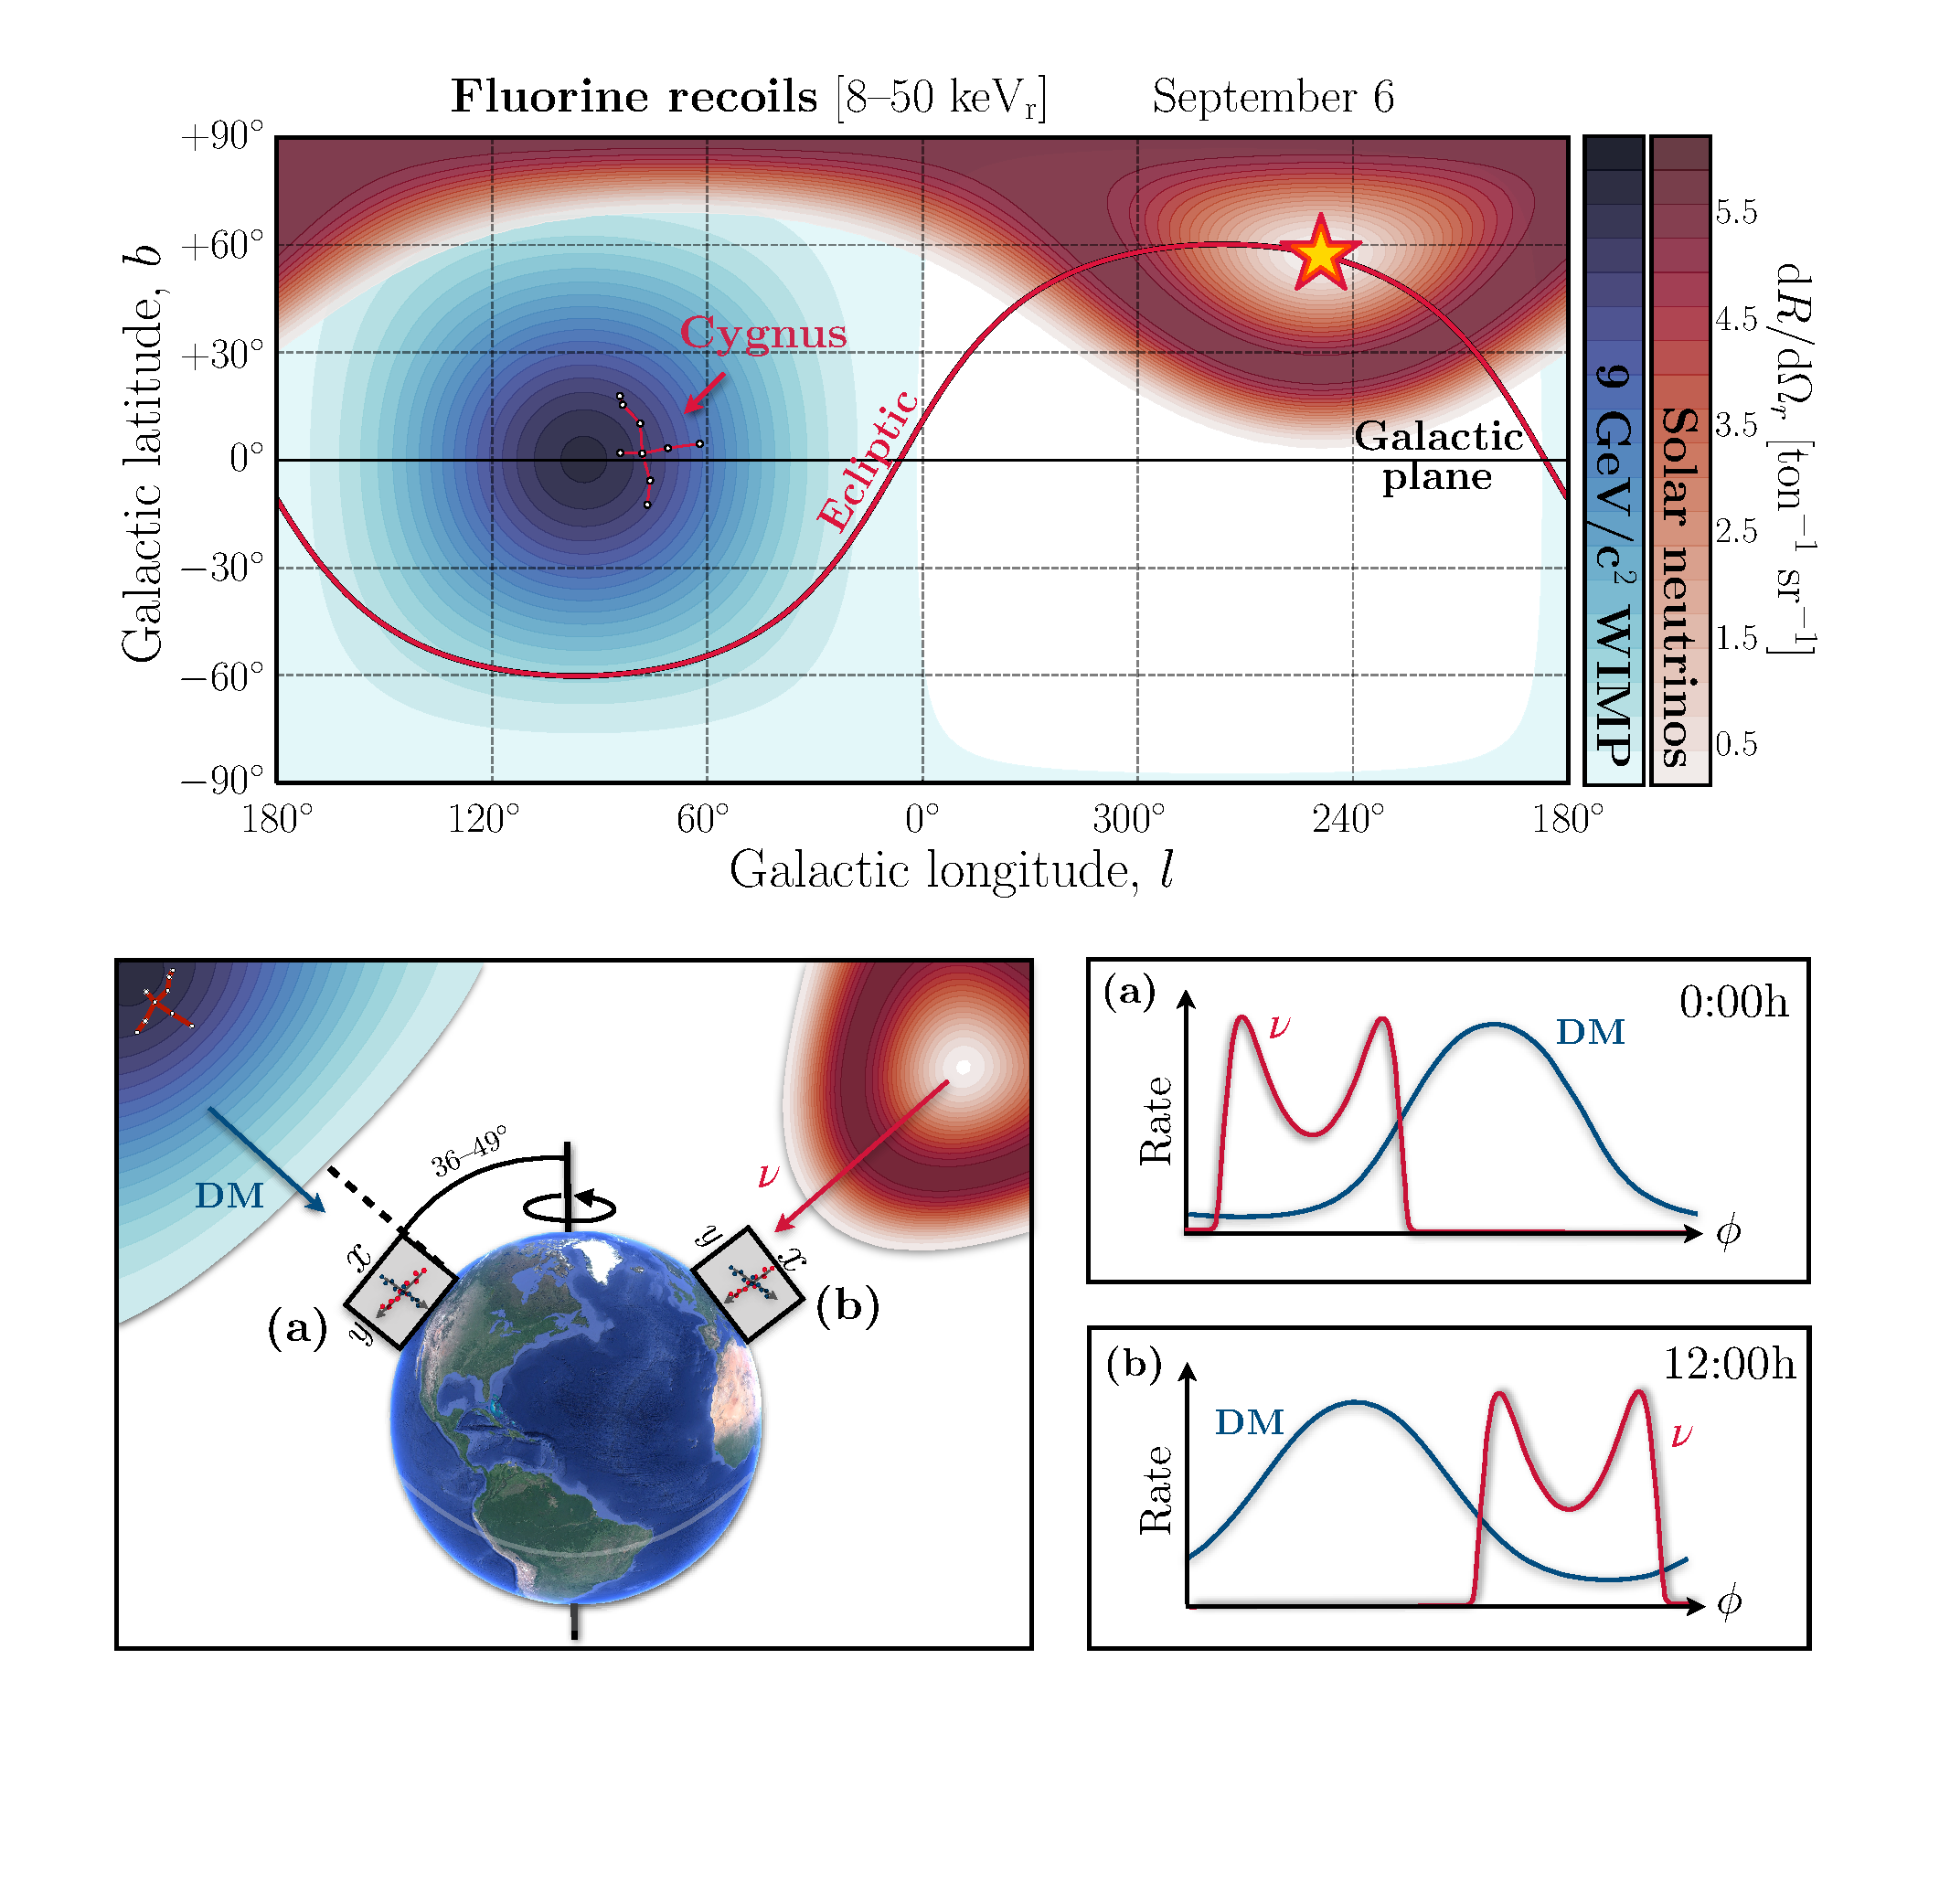
\includegraphics[width=0.99\columnwidth]{figures/Skymaps_extended.pdf}
\caption{The directional DM signature provides strong discrimination against solar neutrino backgrounds. Top: Expected recoil distribution in galactic coordinates. Fluorine recoils from 9~GeV DM particles (blue) form a dipole distribution that always points back to the constellation Cygnus, while the peak of the solar neutrino recoil distribution (red) moves along the Ecliptic throughout the year. Bottom: In lab coordinates, the directional DM and neutrino recoil distributions oscillate out of phase. Figure adapted from Ref.~\cite{Vahsen:2021gnb}}\label{directional_signature}
\end{center}
\end{figure}
 

Most leading direct detection experiments to date, such as the liquid noble gas detectors described above, have primarily aimed to detect Signature 1. This strategy has been highly successful for achieving large exposures at manageable costs, and only a few events are required for a clear detection if the detector remains background free. This method will have reduced sensitivity once exposures reach irreducible backgrounds such as the neutrino fog, or if the background level cannot be reliably predicted. Signature 2 was used by DAMA/LIBRA~\cite{Bernabei:2019ajy} to claim detection of dark matter. This signature can be used even in the presence of backgrounds, but requires exquisite detector stability and a large number (1000s) of observed DM events to detect the relatively small (few-percent-level) modulation magnitude. One important complication is that systematic effects such as temperature and cosmic ray rates also have an annual modulation, casting doubt on any claim of discovery using this signature. Signature 3 requires detectors capable of reconstructing the directions of low-energy nuclear recoils, which is not required for Signatures 1 and 2. Detecting these directions generally requires more complex detectors, increasing cost per unit of exposure. On the other hand, because the majority of recoils are expected to point to a single hemisphere in galactic coordinates, the effect is large, so that few detected DM events are required. Neither radio-impurities nor solar neutrinos can mimic the dipole signature expected from dark matter~\cite{OHare:2015utx}. Being large in magnitude and experimentally robust, the directional dipole signature is the ``smoking gun" signature required to clearly demonstrate that an excess over background in a direct DM detector originates from the galactic halo.

Note that all three methods implicitly rely on the existence of a dark matter halo and $\sim 300$ km/s DM wind when they project and set limits. Moreover the alignment of the dipole is very precisely known thanks to modern astronomical data~\cite{GaiaDR2_disk}. Also note that Signature 3, when viewed in lab coordinates as a large directional oscillation (Fig.~\ref{directional_signature}, bottom), cannot result unintentionally from systematics such as daily temperature fluctuations, because the DM oscillation follows the sidereal day rather than the solar day. That means systematics such as daily temperature and cosmic ray rate fluctuations would oscillate at a different frequency than the DM signal, with the phase difference of the true DM signal and such oscillating backgrounds reaching 180 degrees in six months.

%Directional Lead: Sven Vahsen

\subsubsection{Classes of Directional Detectors}
  
The various strategies for directional recoil detection are reviewed in Ref.~\cite{Vahsen:2021gnb}, and summarized in Fig.~\ref{directional_classification}. Directional detection can be achieved either directly by imaging the nuclear recoil trajectory, or indirectly by inferring the direction from a proxy variable. We will see below that low-density gas TPCs are capable of direct recoil imaging. Examples of the indirect approach include anisotropic light yield in crystals, and anisotropic ionization detection due to columnar recombination in liquid or gas. While the use of solid or liquid targets enabled by indirect techniques at first appears preferable to the gas TPC approach, in order to maximize target mass, to date none of the indirect effects have been clearly observed observed at the low, keV-scale, energies relevant for DM searches.  With a small (order 1\%) effect indirect effect, a prohibitively large number (order $10^5$) of DM interactions would be required to conlusively detect the DM dipole signal~\cite{Vahsen:2021gnb, OHare:2020lva}. Furthermore, indirect directionality typically does not yield independent event-level energy and direction information. That is a disadvantage, as DM detectors that do measure energy and direction independently, can serve the dual purpose of detecting solar neutrinos and reconstructing the incoming neutrino energies event-by-event from the recoil energies and directions. Another draw-back of the indirect method is reduced particle identification (and hence background rejection performance) because less information about the recoil is obtained. For all these reasons, the community working on directional detection is now focusing on detectors where the recoil direction is measured directly, at the event level, by imaging the recoil track. We refer to such detectors as Recoil Imaging Detectors~\cite{SnowmassIF53}.


\begin{figure}[!htbp]
\begin{center}
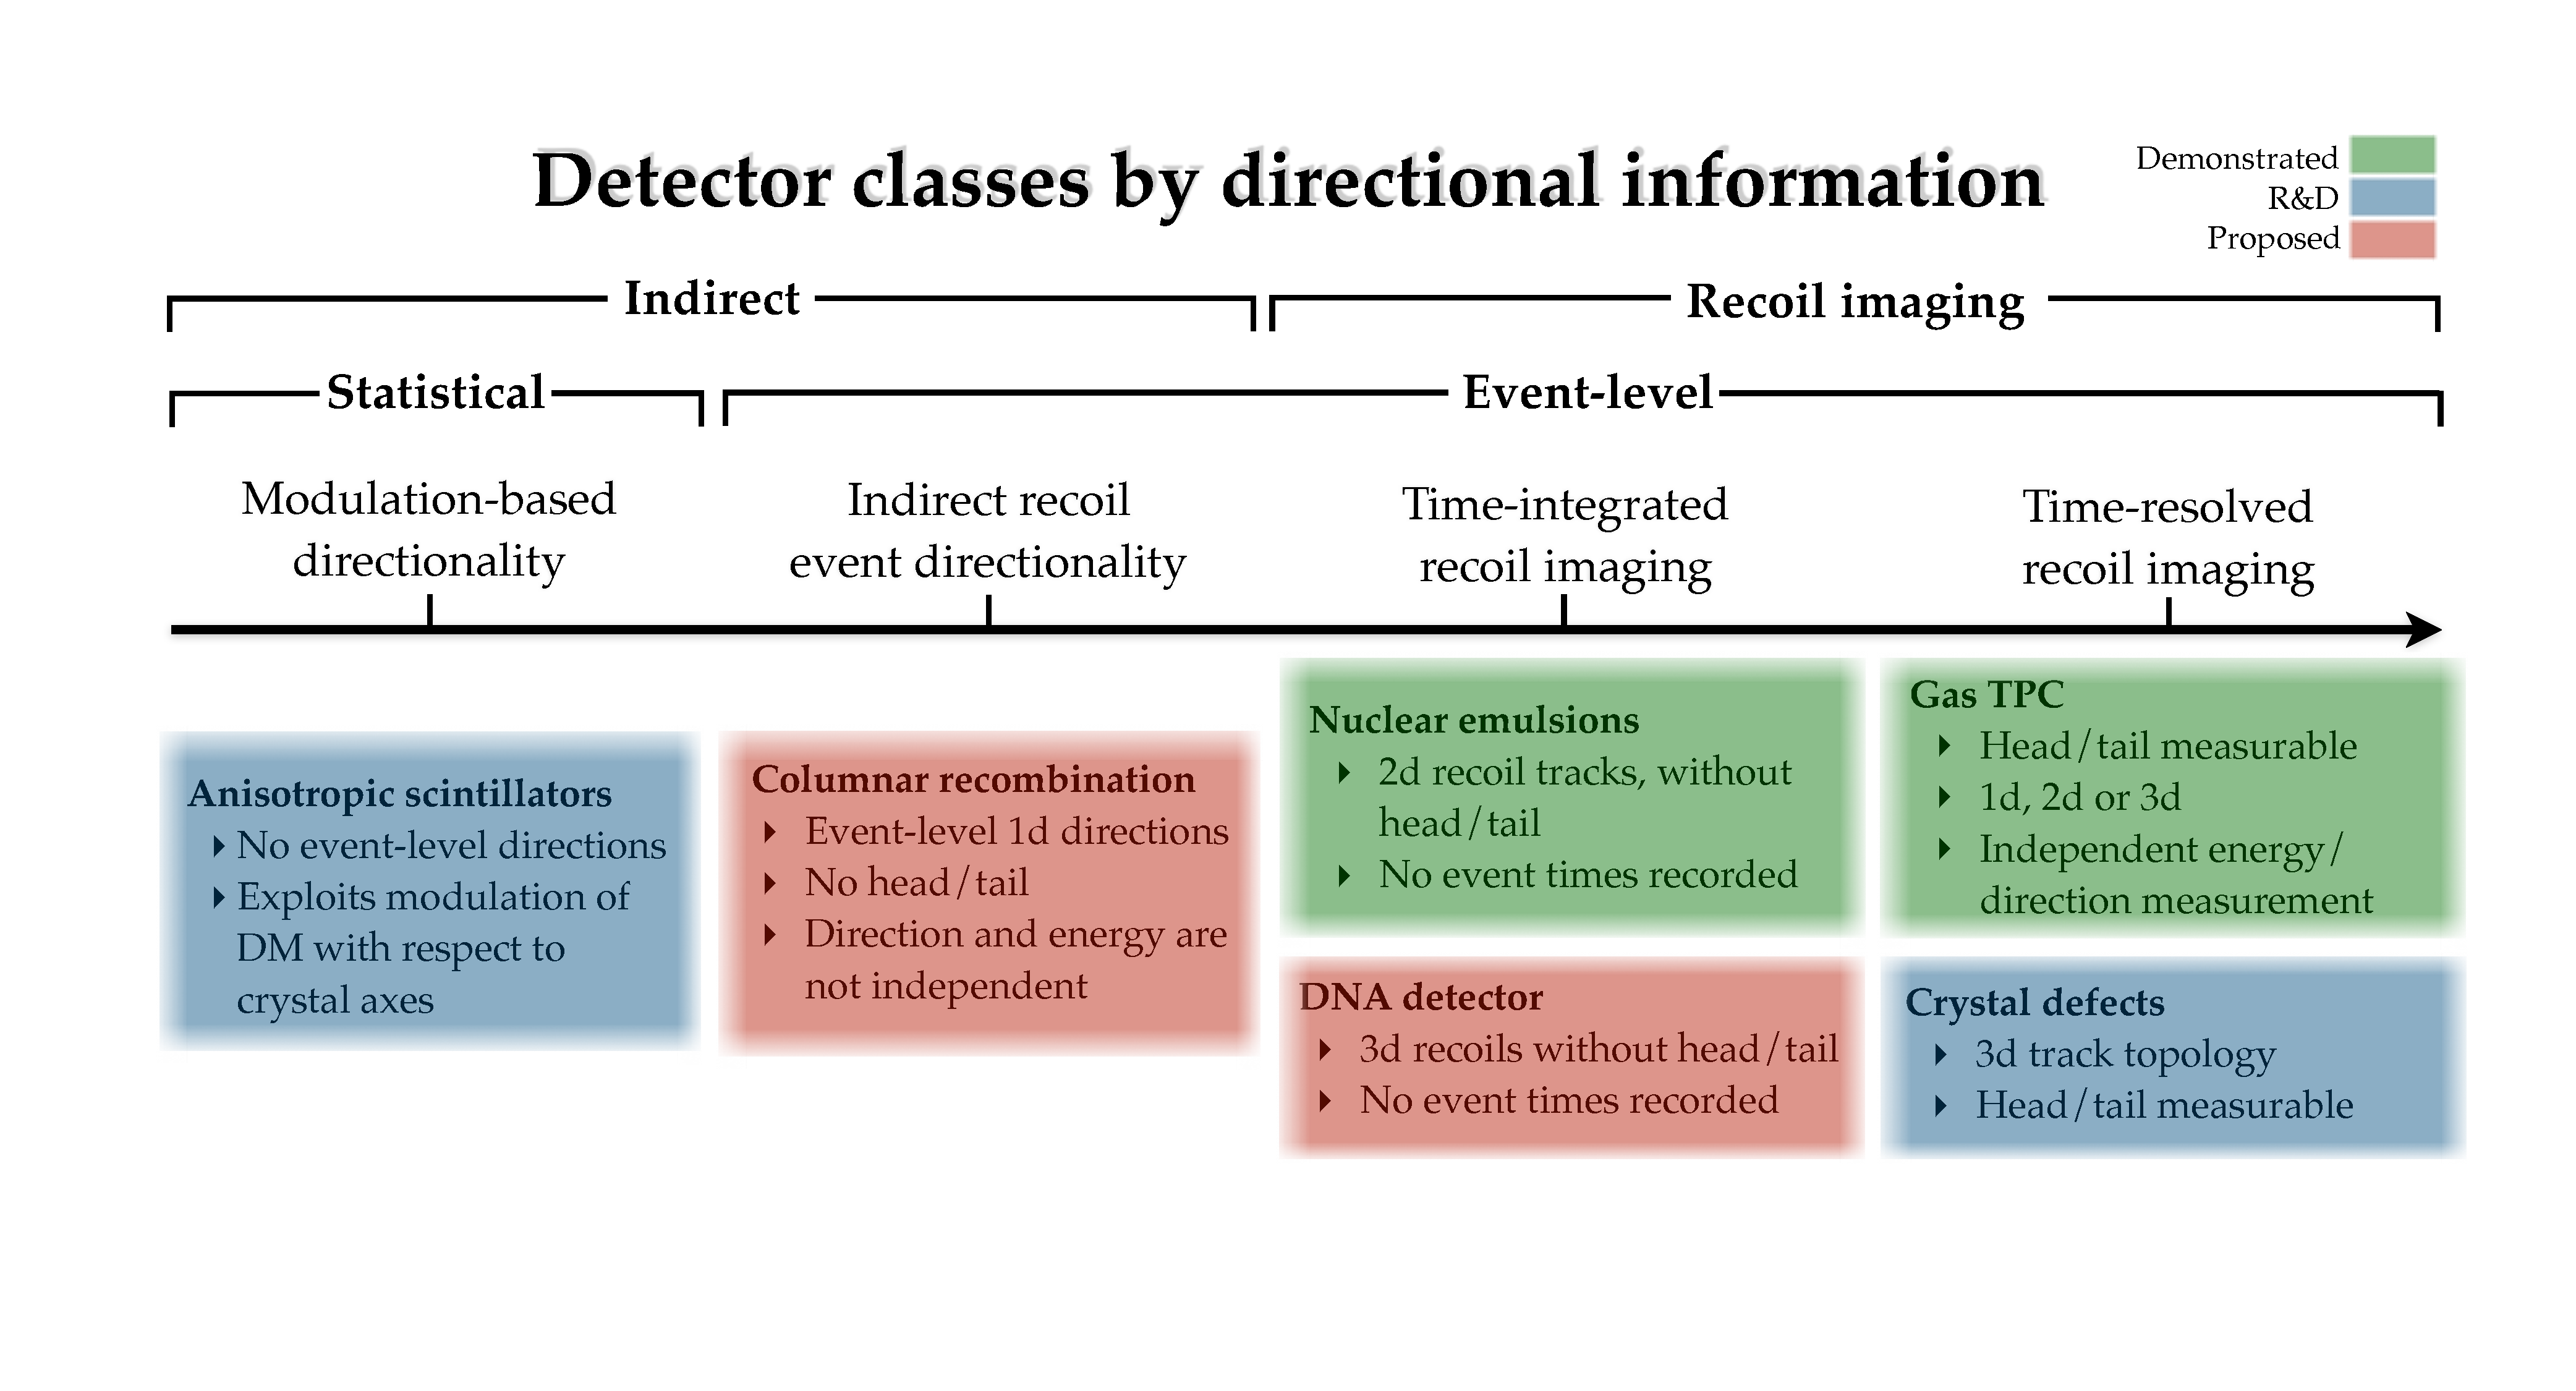
\includegraphics[width=0.99\columnwidth]{figures/DetectorClassTableAR.pdf}
\caption{ Figure adapted from Ref.~\cite{Vahsen:2021gnb}}\label{directional_classification}
\end{center}
\end{figure}

\subsubsection{Directional Detection Performance Requirements}
 
With a recoil-imaging detector, it is possible to observe the directional galactic dipole signature with as few as 5-10 detected DM events. The exact number of events required depends strongly on the detector’s directional performance. For example, to reject a solar neutrino background hypothesis at 90\% C.L., using only the observed angular distribution of recoils, requires less than 10 detected DM events if the performance is at the level of the following or better:

\begin{itemize}
\item recoil axis angular resolution $\leq 30^\circ$ 
\item efficiency for correctly detecting the recoil head/tail $>$ 80\%
\item offline rejection of electron-recoil background by factors $>10^5$. (Estimate for a 1000~${\rm m}^3$ gas TPC~\cite{Vahsen:2020pzb}. For smaller detectors, proportionally smaller rejection factors suffice.
\item fractional energy resolution, $\sigma_E/E$ of order 10\% at 5.9~keV
\item modest timing resolution, of order 0.5~h
\end{itemize}

The key technology challenge in directional detection is to meet the first three requirements at the lowest recoil energy possible, so that the required number of directional events can be detected with the smallest possible exposure.

\subsubsection{Recoil Imaging Technologies}
 
Detecting the direction of low-energy nuclear recoils at this level of accuracy is challenging. In condensed matter, the recoil length scale is order nm. In liquid TPCs where recoil ionization is drifted, electron diffusion is much larger than this recoil length and destroys the directional information. In solid targets, nuclear emulsions have been demonstrated as a means to achieve directional recoil detection. These detectors do not meet the timing requirement stated above, so that event time could not be used to transform the recoil direction into galactic coordinates. Such detectors would therefore have to be mounted on equatorial mounts, continuously rotating the detector to point towards the DM wind, so that the recoil direction always is with respect to the expected dipole direction. This complicates the detector design but is not an inherent showstopper. The NEWS collaboration (based in Japan and Italy) is pursuing directional recoil detection in emulsions~\cite{NEWS:2016fyf} and making good progress. Outside the particle physics community, defect spectroscopy in crystals~\cite{Marshall:2020azl} has been proposed as an alternative method for achieving directionality in solid targets. This work is at the early R\&D stage and would first need to be demonstrated as a viable technique for directional dark matter detection before it can gain traction in particle physics. The remaining world-wide groups working on recoil imaging are therefore pursuing low-density gas TPCs, which they consider the most promising direction. In gas TPC detectors, keV-scale nuclear recoils can be mm in length, while charge diffusion is of order 100~$\upmu$m. This allows the ionization from low-energy nuclear recoils, and hence recoil directions, to be reconstructed in detail. Recently, virtually all of the groups worldwide that are pursuing directional detection in gas TPCs joined forces to form the CYGNUS Detector R\&D collaboration.

\subsubsection{Quantum defects in wide-bandgap semiconductors}
 Quantum defects in wide-bandgap semiconductors are also proposed to achieve directional sensitivity at solid-state densities \cite{Rajendran:2017ynw,Marshall:2020azl, the snowmass whitepaper}. Event registration under this proposal would use technologies developed for DM detection in semiconductor targets, which yield the event time and mm-scale position. The incident particle's direction would be stored as a durable, submicron track of crystal lattice damage, which could be mapped using solid-state quantum sensing methods. Early R\&D has focused on nitrogen-vacancy defects in diamond \cite{Marshall:2020azl,Marshall:2021kjk,Marshall:2021xiu} to establish the feasibility of directional readout of such tracks. If successful, this will motivate further collaboration between the particle physics and solid-state quantum sensing communities toward DM detectors with sensitivity below the neutrino fog.
 
\subsubsection{CYGNUS}
 
The CYGNUS collaboration proposes to build a $\ge 1000~{\rm m}^3$ recoil-imaging gas target TPC. The proposed detector consists of a large number of smaller modules, which allows for the large volume to be distributed across multiple underground laboratories. Gas detectors have lower target mass per unit volume than liquid or solid target detectors, which is a clear disadvantage for DM searches. However, modern gas TPCs can detect even individual electrons of ionization with $\mathcal{O}(100~\upmu$m) spatial resolution, which is shorter than the nuclear recoil length, and enables directionality. Gas TPCs can be scaled to large volumes at reasonable cost without degrading performance, by using a modular structure where each module has a short, $\mathcal{O}$(50 cm), drift length. The unique directional capabilities of gas TPCs may outweigh their low target density once their cost is reduced sufficiently, when irreducible backgrounds appear, or if other physics can be performed. All three of these conditions are now met: 1) In recent years, micro-pattern gaseous detectors (MPGDs), developed by the RD51 collaboration at CERN for LHC experiments, have greatly reduced the cost of highly segmented TPC charge readout planes. As a result, recoil imaging gas TPCs are now realistic at a cost of order \$10k per cubic meter. This means even a 1000~m$^3$-scale observatory is at the \$10M cost scale, i.e. of similar cost as that of a single detection system in a large particle physics experiment. 2) We are rapidly approaching the neutrino fog, so that DM detectors are guaranteed to see an irreducible background. This is a background which can be clearly separated from DM signals via directionality. 3) The neutrino scattering events expected in the neutrino fog can also be exploited as a signal. Interestingly, already a much smaller, order 10~m$^3$ TPC module can do interesting solar neutrino measurements by also utilizing electron recoils. For a given neutrino energy, the electron recoils have much higher recoil energy but lower ionization density than nuclear recoils, and are readily observable in a low-threshold gas TPC, with directionality.

\begin{figure}[!htbp]
\begin{center}
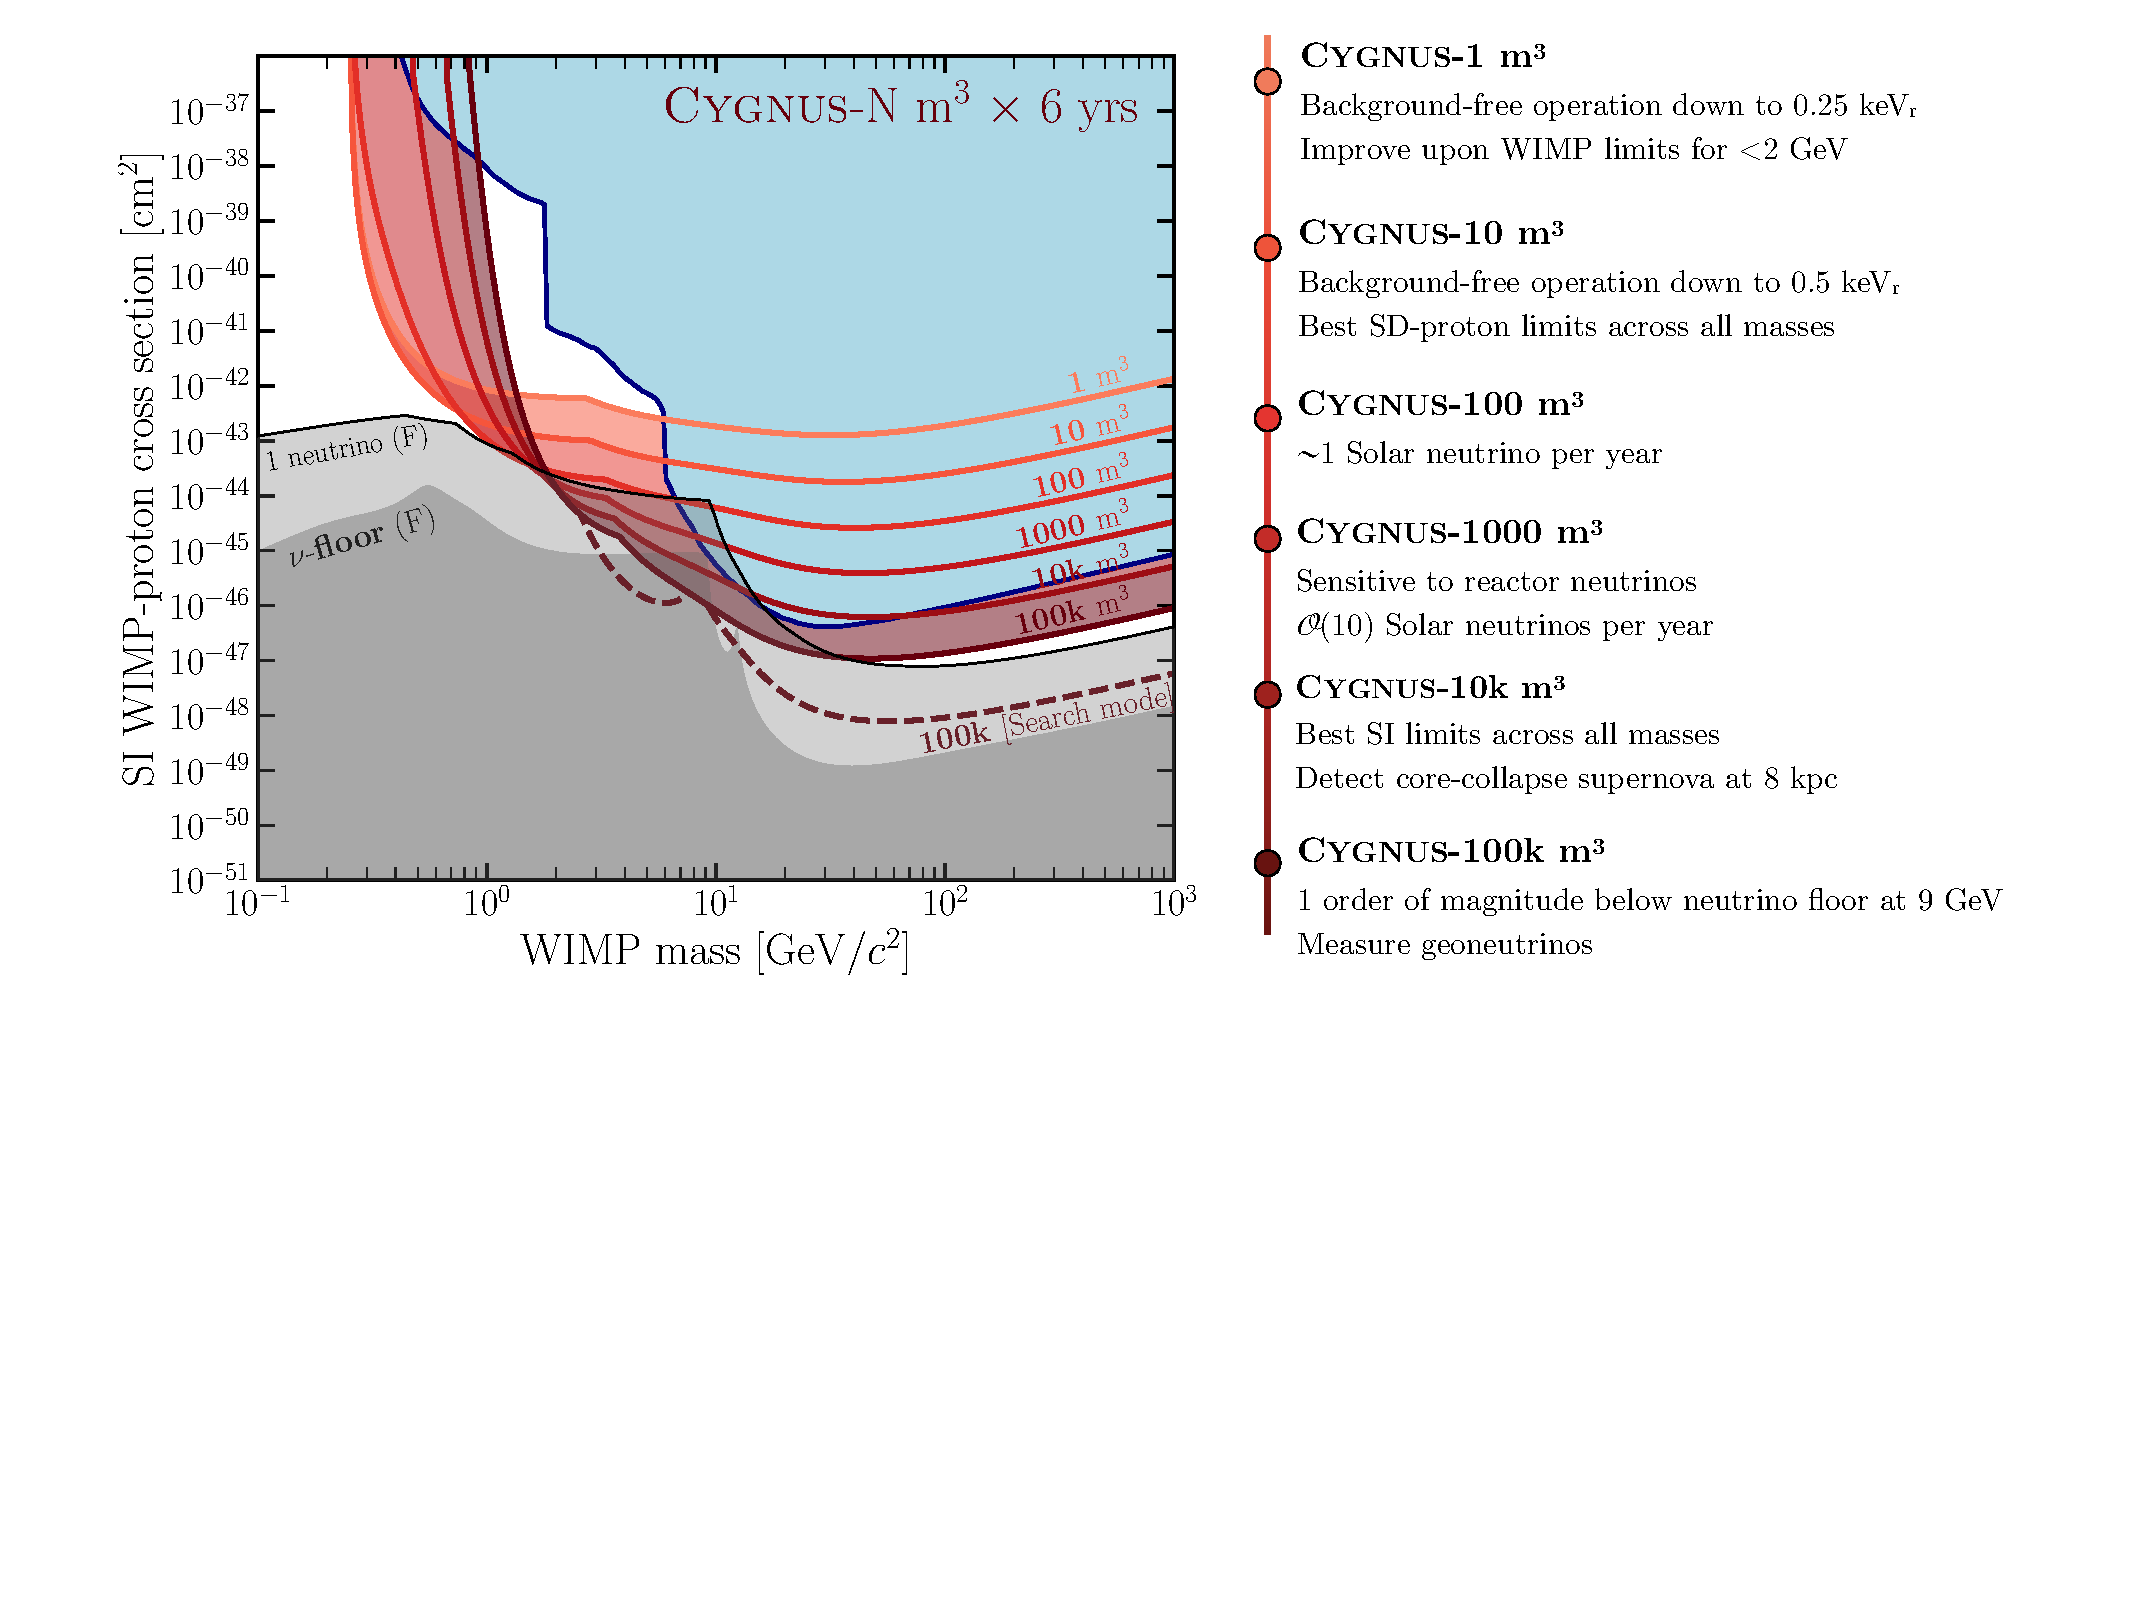
\includegraphics[width=0.99\columnwidth]{figures/Cygnus_listed_timeline.pdf}
\caption{Projected SI WIMP-proton scattering cross section 90\% CL exclusion limits for various CYGNUS fiducial volumes, each for 6 years of exposure, for a He:SF$_6$ (755 Torr : 5 Torr) fill gas. Currently excluded limits on the SI DM-nucleon cross section are shaded blue. The CYGNUS thresholds are increased evenly from 0.25 to 8 keVr for each increasing volume to reflect the range of possible thresholds of the final experiment. There is a factor 30 reach improvement possible if a non-directional ``search mode" fill gas such as 1520 Torr of SF$_6$ is used. We show this only for the largest scenario, but this option exists at every scale. Figure adapted from \cite{Vahsen:2020pzb}.\label{cygnus_timeline}}
\end{center}
\end{figure}

A plethora of other physics can be performed with a modest-volume, high-resolution gas TPC experiment. The staged program above will provide both competitive measurements of known phenomena, such as solar neutrinos, and unique searches for physics beyond the standard model, in the form of particle dark matter or non-standard neutrino interactions.  More details, including additional DM reach curves and expected neutrino event counts, can be found in a designated Snowmass White Paper~\cite{SnowmassIF53}, in a recent review of the field~\cite{Vahsen:2021gnb}, and in a concept paper describing the proposed CYGNUS experiment~\cite{Vahsen:2020pzb}. Figure~\ref{cygnus_timeline} shows the directional CYGNUS DM reach versus volume, for the potential target gas He:SF$_6$ (755 Torr : 5 Torr). Because the design and gas choice are not final, these reach curves are likely to change, possibly substantially, in the future.


%FIXME add #expected neutrino events here for some example gases?

The approximate timeline for CYGNUS worldwide is:
\begin{itemize}
\item 2022-2025: 1~m$^3$ detectors to be constructed and start operation in the UK, Japan, Italy, US, and Australia. The US detector may be used above-ground for CE$\upnu$NS measurements at a neutrino beam.
\item 2025-2035: 10~m$^3$ detectors: CYGNUS HD10 module (electronic readout) to be jointly constructed + operated in the US. A CYGNO detector (optical readout) program is planned and funded in Italy. Detectors in Japan, the UK, and Australia are also planned.  
\item 2024-2042+: 1000~m$^3$ detectors: design of $\ge$1000~m$^3$ facility with 10~m$^3$ modules to start in 2024. If the project remains successful, construction of a 1000~m$^3$ facility will begin in 2030.
\end{itemize}

\paragraph{CYGNUS HD in the US: Recoil Directionality below 10~keV}

The largest directional DM detector prototypes to date have been 1~m$^3$ in volume, and were built by the DRIFT and DMTPC collaborations. These early efforts were important in exploring two main approaches to the target gas, negative ion versus electron drift, and to the TPC readout, electronic versus optical. Both detectors were designed to search for 100-GeV DM particles, and have limited directionality for recoil energies below 50~keVr. Several hundred detected events would be required for a directional DM discovery with DRIFT. Recently, however, smaller R\&D detectors in the US have shown that the particle identification and event-level recoil directionality required for a directional discovery with only 5-10 events can be achieved even at sub-10-keV energies with modern MPGD-based detectors.

\begin{figure}[!htbp]
\begin{center}
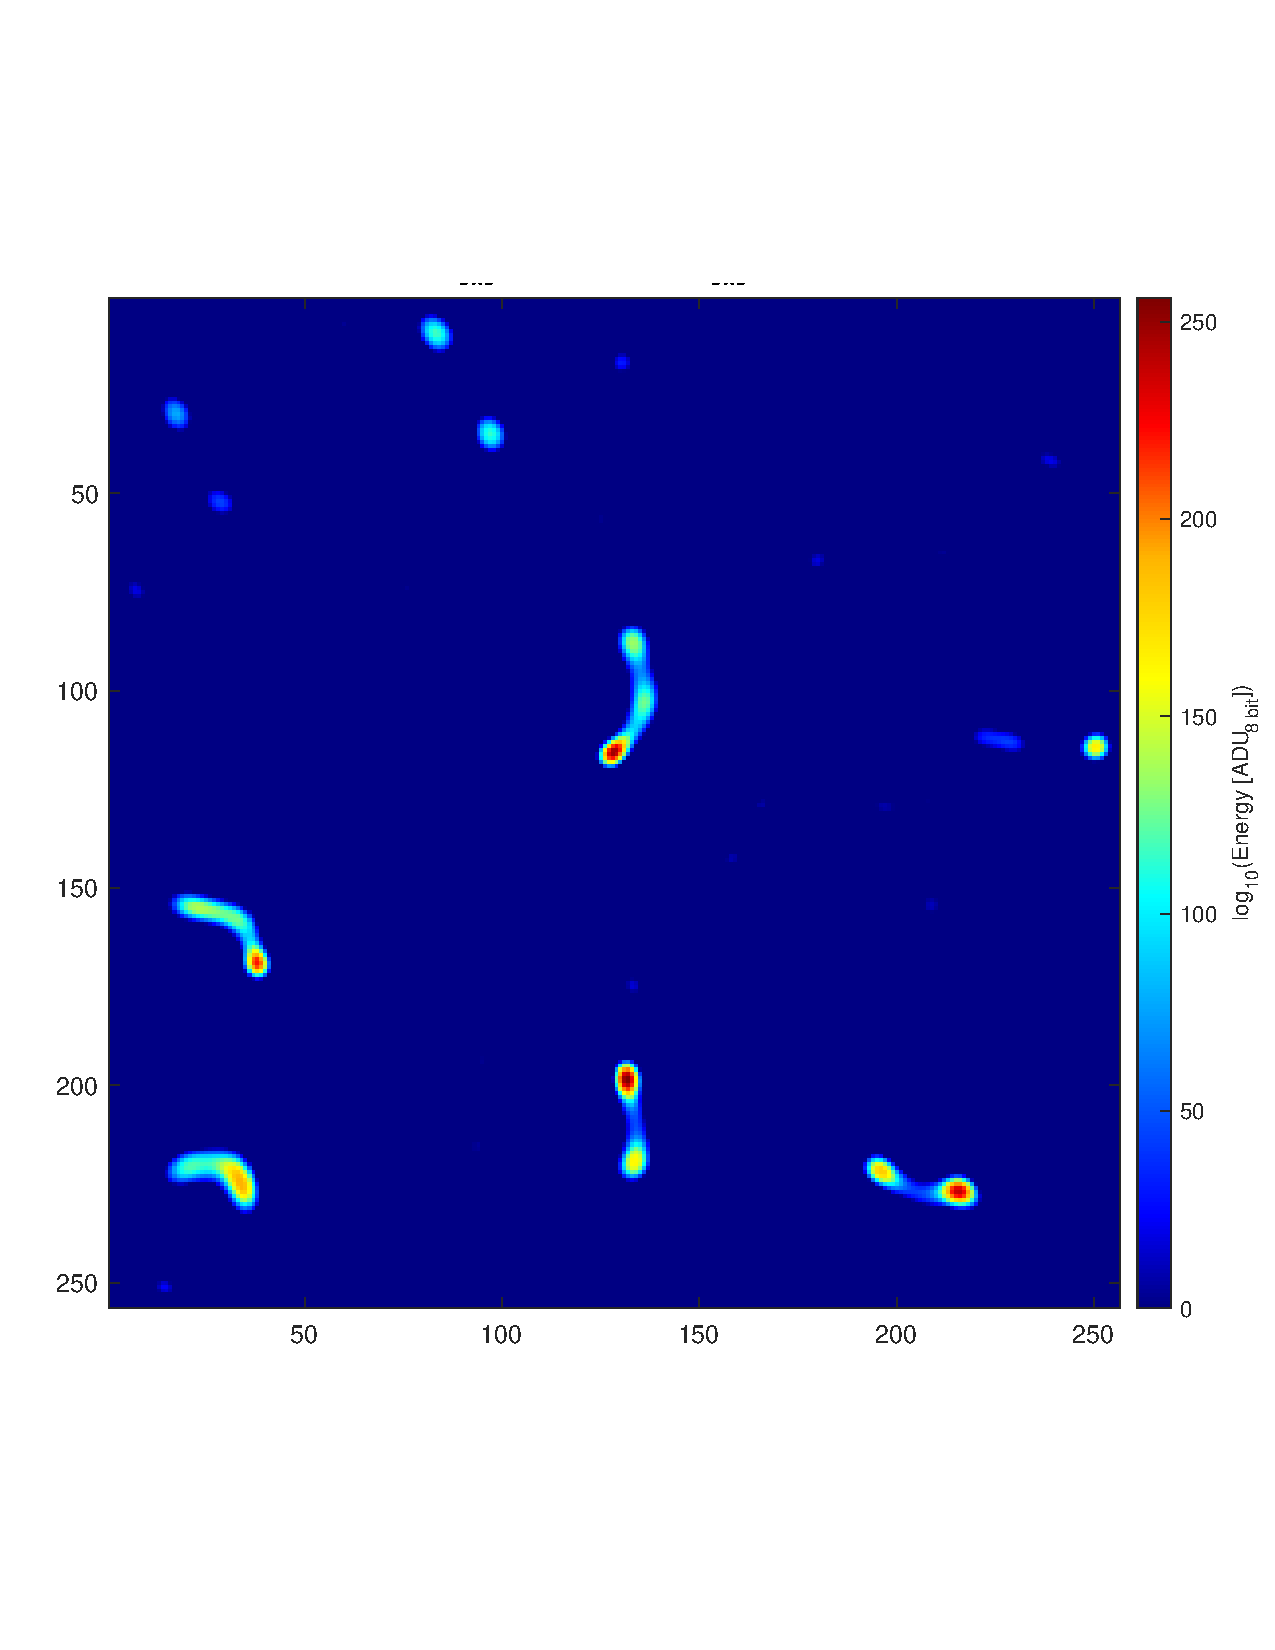
\includegraphics[width=0.49\columnwidth]{figures/optical_Fe55.pdf}
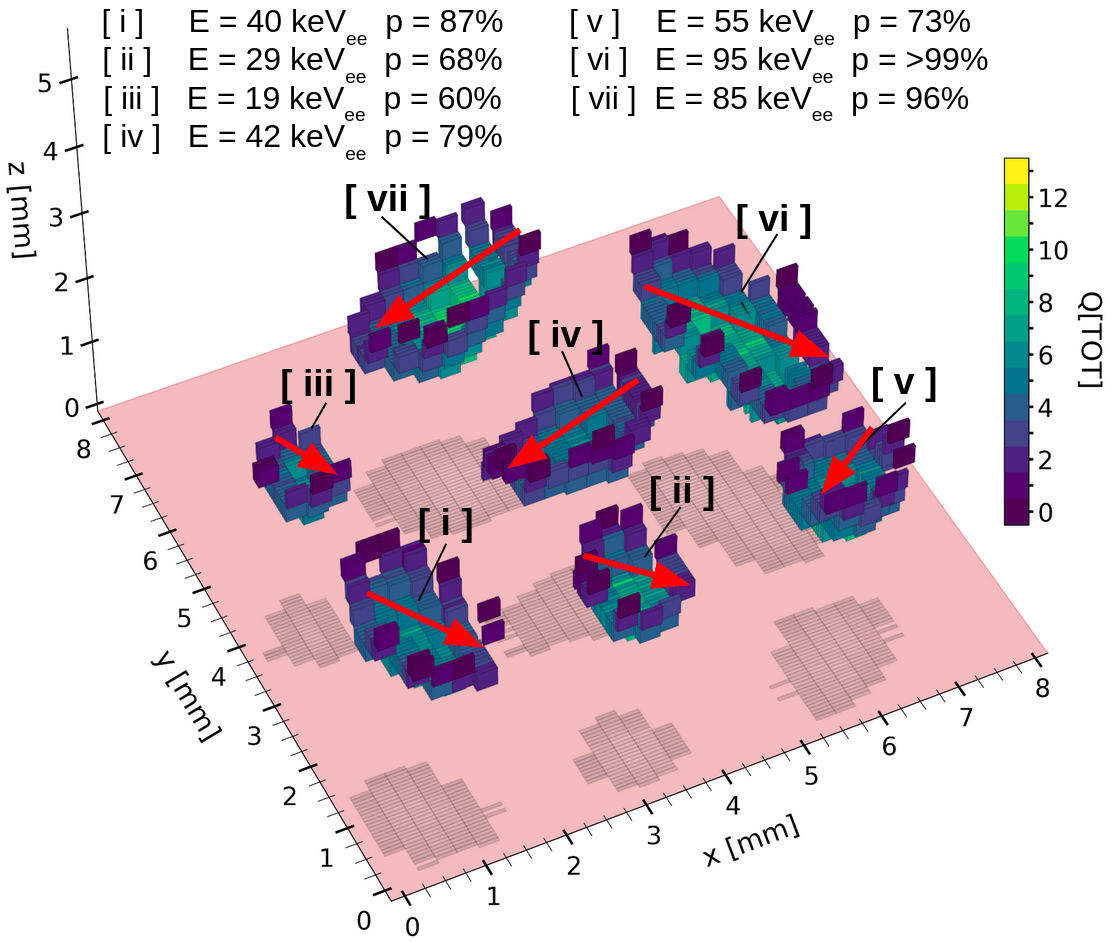
\includegraphics[width=0.49\columnwidth]{figures/BEAST_logain.png}
\caption{Experimental data from TPCs with MPGD readout. Left: 5.9~keV electron events in a 2D optical-readout TPC with GEM amplification at U. New Mexico. The fill gas is 30 Torr CF$_4$, the drift length is 2~cm, the gain $10^5$, the pixel size is $175 \times 175~\upmu$m$^2$. Deconvolution has been applied. Right: Helium-recoils induced with a neutron source, in a 3D electronic-readout TPC with GEM amplification at U. Hawaii. The fill gas is 760 Torr He:CO$_2$ (70:30), the drift length is 11~cm, the gain is ~$900$, the 3d voxel size is $50 \times 250 \times 250~\upmu$m$^3$. Raw data is shown, without any post-processing. The red arrows show fitted recoil directions, with the head and tail (i.e. sign of the vectors) determined by a 3d convolutional neural network. The confidence level of correct assignment is indicated in the legend. }\label{gas_tpc_events}
\end{center}
\end{figure}

Figure~\ref{gas_tpc_events} shows examples of electronic and nuclear recoil events recorded in state-of-the art ``CYGNUS HD'' TPC prototypes at US institutes. Advantages of optical readout include high segmentation and off-the-shelf, commercially available DAQ systems. Pixel ASIC readout is the most sensitive gas TPC readout technology, and enables 3d imaging. The events shown in Fig.~\ref{gas_tpc_events} (right) were recorded at low gain, only about 900, where electron recoils are strongly suppressed due to their lower ionization density. However, these detectors~\cite{Jaegle:2019jpx} operate stably at gains of at least $5\times 10^4$. Depending on the charge threshold used, at gains exceeding 3000-9000, single electrons of primary ionization are detected with high efficiency. Events recorded in single-electron mode are shown in Figure~\ref{single-electron}. The ionization threshold in this case is order 30~eV, and Sub-10-keV recoils are easily detectable as large signals compared to a negligible background from noise hits.


\begin{figure}[!htbp]
\begin{center}
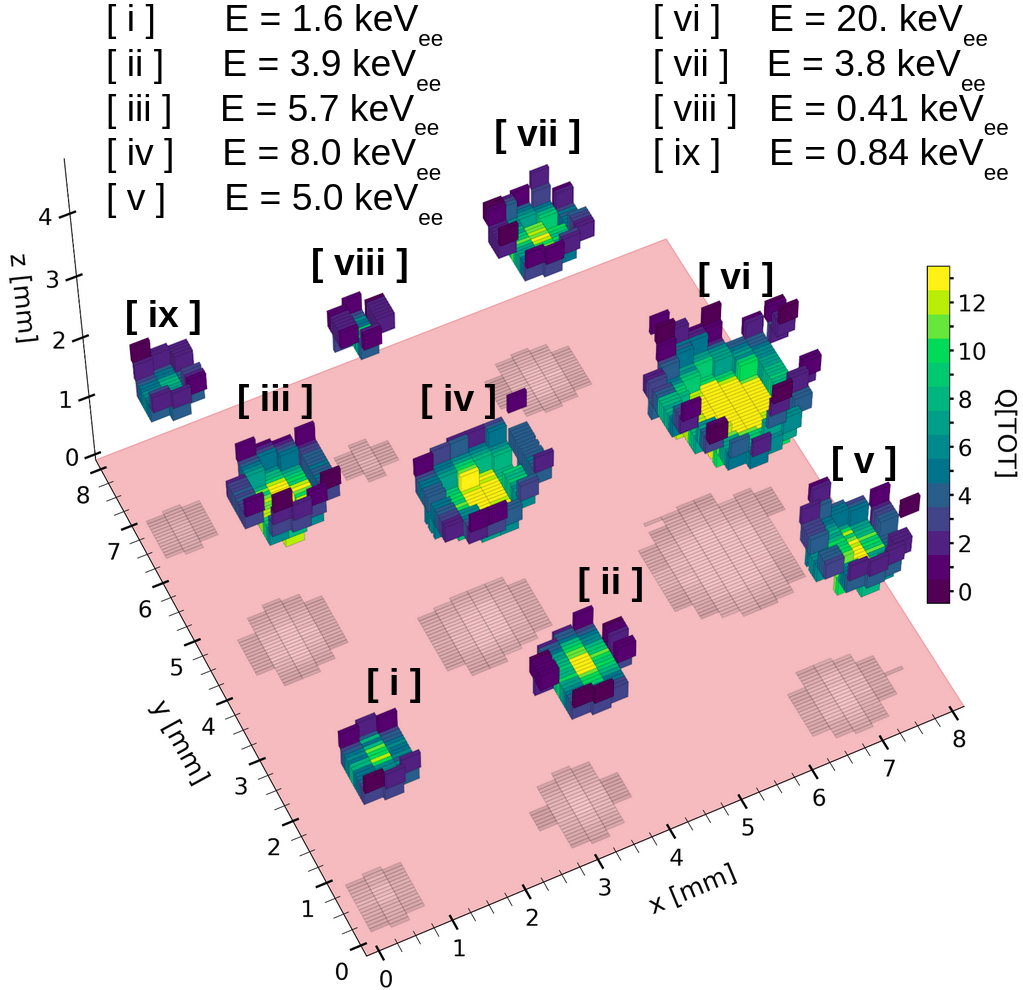
\includegraphics[width=0.49\columnwidth]{figures/BEAST_higain.png}
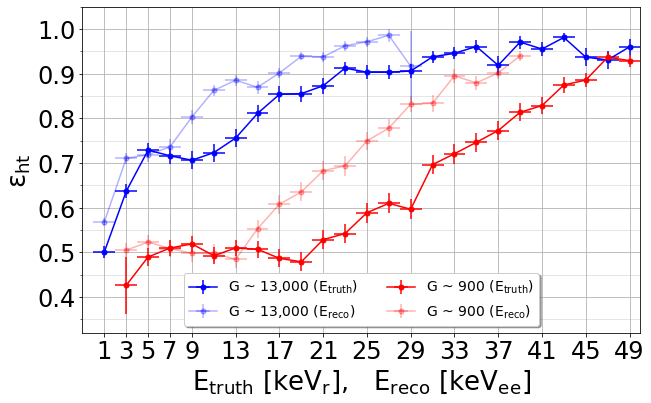
\includegraphics[width=0.49\columnwidth]{figures/headtail.png}
\caption{Left: Nuclear recoils detected in a pixel-ASIC TPC operating in the single-electron regime, at a gain of $1.3\times 10^4$. Right: Head/tail efficiency for helium-recoils versus energy, obtained with 3D convolutional neural networks on simulated pixel-ASIC TPC data for two different gas avalanche gain settings. }\label{single-electron}
\end{center}
\end{figure}

To utilize this type of extreme sensitivity in directional DM searches, the detectors themselves are not sufficient. We must also separate electronic and nuclear recoils, and assign recoil directions, even at the lowest observed energies. This challenge has motivated novel algorithm development for low-energy particle identification and head/tail detection over the last few years. CYGNUS HD recently achieved both the desired low-energy particle identification and directional capabilities with 3D convolutional neural networks (3D CNNs). Figure~\ref{single-electron} right shows the head/tail correct assignment efficiency in a pixel TPC, versus recoil energy. At low gain (\~900), the desired 70\% head/tail efficiency is obtained only down to 20~keVee in simulation, while in high-gain (single-electron) mode, this performance is extended down to 3keVee. The low-gain performance has already been confirmed experimentally. The high-gain experimental data is currently being analyzed.

These recent developments are extremely promising. However, we expect substantial further improvements: the event displays and 3~keVee directional threshold seen in Fig.~\ref{single-electron} is obtained with an electron drift (i.e. high diffusion) gas at atmospheric pressure. Both choices reduce low-energy directionality. Also, the detector utilizes a double-GEM gain stage which limits the point resolution. The result is that the sub-10~keV recoils appear round to the eye, even though the CNN can still determine the head/tail in this regime. A CYGNUS feasibility study~\cite{Vahsen:2020pzb} suggested that Micromegas amplification integrated with 2D x/y strip readout is a cost-optimal way to improve the low-energy performance even further, and to scale directional detectors up to very large volumes. Because of reduced charge sharing across fewer pixels in a micromegas-based detectors compared to GEM-based detectors, the gain required for single-electron detection is reduced by a factor of ~5. Then, it should be feasible to detect single electron even when using negative ion drift, where gains are reduced. The negative ion drift would in turn minimize diffusion, while the electron counting would remove the contributions of gain-fluctuations to the energy resolution. The expected end results would be a CYGNUS detector operating at the fundamental performance limit, where individual primary electrons are counted in 3d at $100~\upmu$m$^3$ spatial resolution. Recent R\&D with GridPix charge readout ~\cite{Ligtenberg:2021viw} has demonstrated the feasibility of this on a smaller scale. The CYGNUS HD members in the US are currently building prototypes to demonstrate sub-10-keV directionality at the 40~l and then 1000~l module scale. For further detail, we refer the reader to Refs.~\cite{Vahsen:2021gnb,Vahsen:2020pzb}. 







\subsection{EFT couplings}
Lead: David Cerdeno

For the N most basic EFT couplings, What is the currently-excluded cross section from published results?  \textbf{Is there a mass range that is not being probed in one or more couplings?} Are there new technologies that uniquely address some portion of this parameter space?

\begin{figure}
    \centering
    %\includegraphics{}
    \missingfigure[figheight=16cm]{EFT cross section space excluded}
    \caption{7 or so plots of current and near-future EFT cross-section sensitivity.}
    \label{fig:EFT_sensitivity}
\end{figure}


% Prisca: I suppose our charge is to the neutrino floor. Are ER searches the only thing getting there (under our charge)?   Do we cover only electron scattering (elastic and inelastic) and NOT dark sector stuff and dark photon absorption?   What about getting to the neutrino floor at low mass? This is kind of interesting, because the neutrino floor focus could move the discussion away from pushing to the lowest threshold and open up and interesting examination of what the real limit is to low mass at the largest exposures. Thus, a better organizational principle might be for mass regions instead of NR vs ER.  The theory might be easier to subdivide, too.   But if not, I tried to subdivide ER without low mass. 